\subsection{Flächen und Volumen}

\subsubsection{Flächeninhalt zwischen Kurve und \(x\)-Achse}

Bei der Berechnung von Flächeninhalten muss man vorsichtig sein und sich klarmachen, welche Teile der Fläche beim Integral positiv und welche negativ gezählt werden.

\begin{bsp}
	{Musterbeispiel zur Flächenberechnung}{}
	Bestimmen Sie den Inhalt der endlichen Fläche, die von der Kurve \(y=x^3-x^2-6x\) und der \(x\)-Achse eingeschlossen wird.
	\vspace{16cm}

\end{bsp}

\clearpage
\begin{ueb}{Flächen unter Graphen von Polynomfunktionen}{}
	\begin{enumerate}
		\item Bestimmen Sie den Inhalt der endlichen Fläche, die von der gegebenen Kurve und der \(x\)-Achse eingeschlossen wird.
		      \begin{enumerate}
			      \item \(y=x^2-5x+4\)
			      \item \(y=x^3-2x^2-3x\)
			      \item \(y=x^4-10x^2+9\)
		      \end{enumerate}
		\item Der Graph der Funktion \(f(x) = ax-x^3\) schliesst im 1. Quadranten mit der \(x\)-Achse eine Fläche mit dem Inhalt \(A=9\) ein. Berechnen Sie \(a\).
		\item Der Graph einer Funktion 3. Grades hat in \(P=(1, 0)\) die Steigung \(m=1\) und berührt die \(x\)-Achse im Ursprung. Bestimmen Sie den Inhalt der endlichen Fläche zwischen dem Graphen und der \(x\)-Achse.
		\item Der Graph einer Funktion 3. Grades berührt die \(x\)-Achse im Ursprung, hat ein Extremum bei \(x=2\) und schliesst im 1. Quadranten mit der \(x\)-Achse eine Fläche mit dem Inhalt \(A=27\) ein. Bestimmen Sie die Funktionsgleichung und die Koordinaten des Wendepunktes.
	\end{enumerate}
\end{ueb}
\begin{ueb}{Flächen unter Graphen von allgemeinen Funktionen}{}
	\begin{enumerate}\setcounter{enumi}{4}
		\item Berechnen Sie den Inhalt der endlichen Fläche, die von der Kurve \(y=\sqrt{x}-\frac{1}{2}x\) und der \(x\)-Achse berandet wird.
		\item Welchen Inhalt hat die Fläche, die begrenzt wird von der \(x\)-Achse, der Kurve \(y=\sqrt{x}\) und der Normalen im Kurvenpunkt \(P=(4, y_p)\)?
		\item Bestimmen Sie den Inhalt eines der (unendlich vielen) Flächenstücke, die zwischen dem Graphen der Funktion und der \(x\)-Achse liegen:
		      \begin{enumerate}
			      \item \(f(x) = \sin(x)\)
			      \item \(f(x) = \sin(x) - \cos(x)\)
		      \end{enumerate}
		\item Bestimmen Sie den Wert der Parameters \(a>0\), sodass die Funktion \(f(x) = (a-x)\cdot \sqrt{x}\) mit der \(x\) Achse eine Fläche mit dem Inhalt \(A=64.8\) einschliesst.
		\item Bestimmen Sie den Inhalt der endlichen Fläche, die von der Kurve \(y=\frac{x^2-5x+4}{x}\) und der \(x\)-Achse eingeschlossen wird.
	\end{enumerate}
\end{ueb}

\clearpage
\emph{Lösungen:}
\begin{enumerate}
	\item Flächenberechnung
	      \begin{enumerate}
		      \item \(A=\frac{9}{2}\)
		      \item \(A= \frac{71}{6}\)
		      \item \(A=52.26\bar{6}\)
	      \end{enumerate}
	\item \(a=6\)
	\item \(f(x)=x^3 - x^2\); \(A=\frac{1}{12}\)
	\item \(f(x)= -4x^3+12x^2\),  Wendepunkt: \(W=(1, 8)\)
	\item \(A=\frac{4}{3}\)
	\item \(A=\frac{35}{6}\)
	\item Flächenberechnung mit trigonometrischen Funktionen:
	      \begin{enumerate}
		      \item \(A=2\)
		      \item \(A=2\sqrt{2}\)
	      \end{enumerate}
	\item \(a=9\)
	\item \(A=1.95\)
\end{enumerate}













































\clearpage
\subsubsection{Die Fläche zwischen zwei Graphen}

Im Folgenden werden Sie lernen, wie man Flächeninhalte von Gebieten berechnen kann, die von zwei Funktionsgraphen begrenzt sind. Dabei gilt die folgende Grundidee:
\begin{satz}
	{Der Satz des toten Wals}{}
	Das Volumen eines Walfs ändert sich nicht, wenn er stirbt.
\end{satz}
Was damit gemeint ist, sehen wir im folgenden Beispiel.
\begin{bsp}
	{Walfang}{}
	Gegeben sind die beiden Funktionen \(f(x)=x^2-2\) und \(g(x)=-x^2+4x-2\). Gesucht ist den Inhalt der Fläche, zwischen den Graphen.
	\begin{center}
		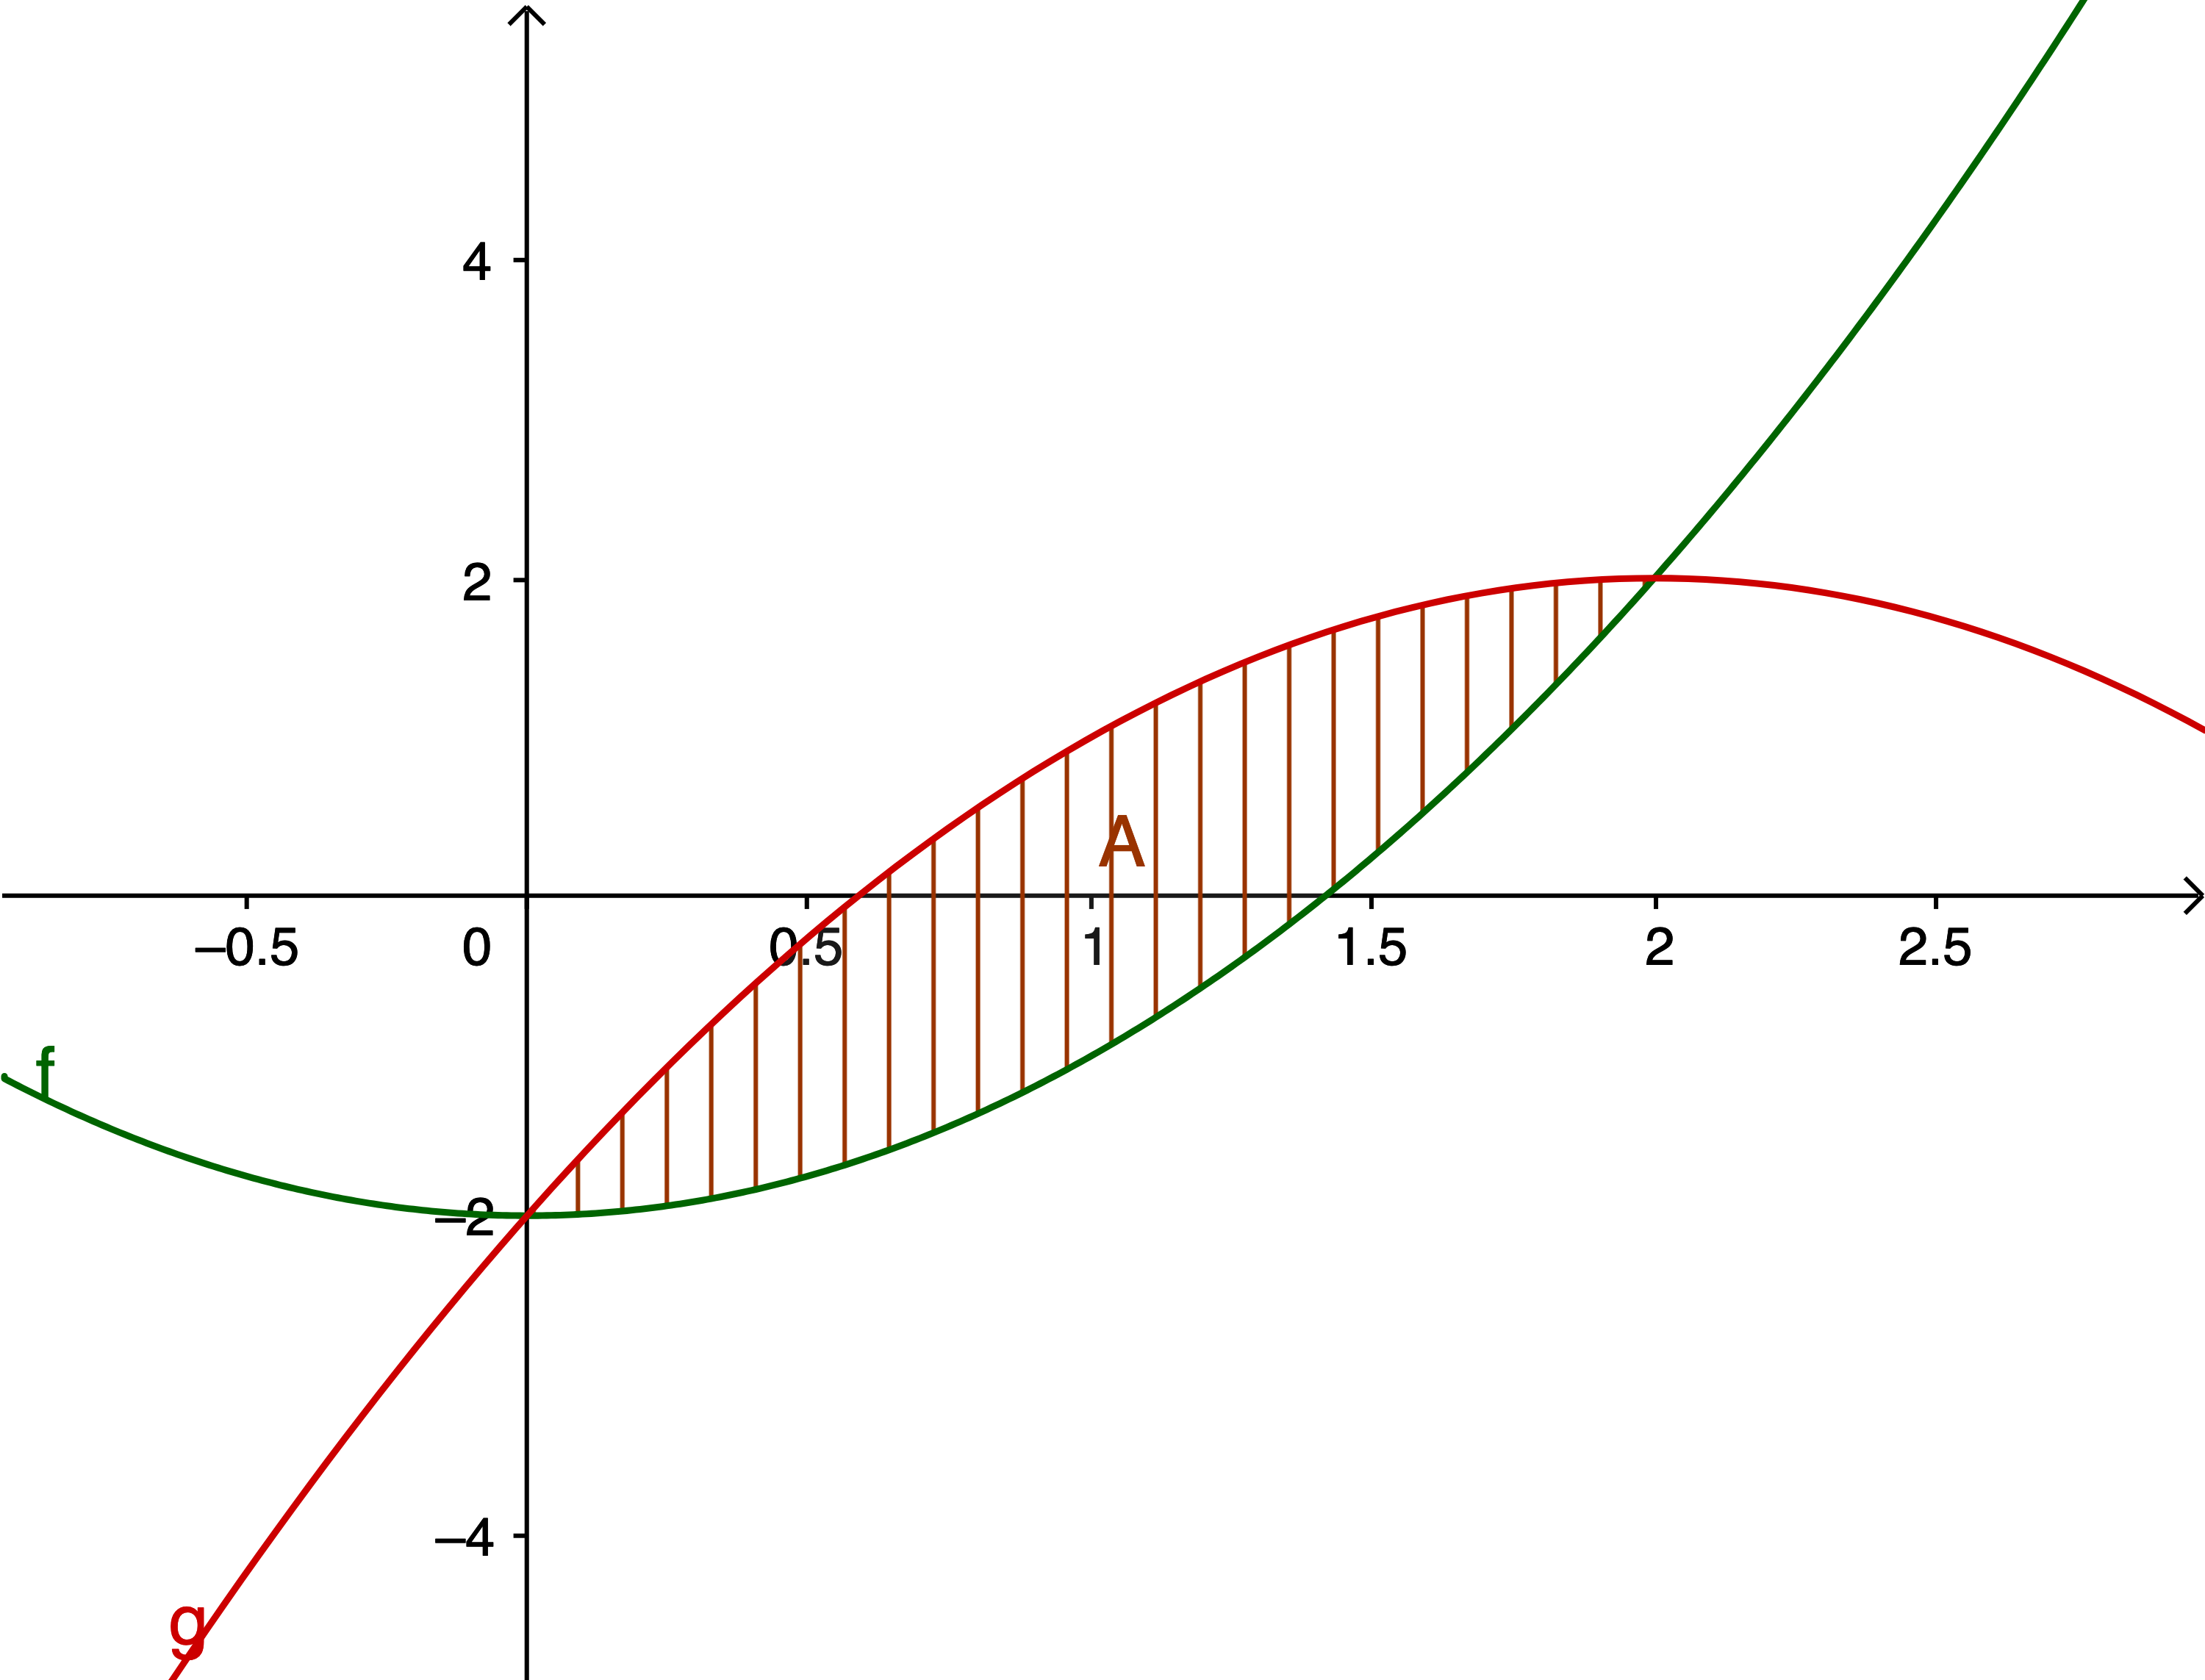
\includegraphics[width = 0.5\textwidth]{media/wal-lebend.png}
	\end{center}
	Die Fläche steht für den lebenden Wal, der durch die Ozeane schwebt. In dieser Lage liegt die Berechnung des Flächeninhalts nicht auf der Hand. Aber es wird einfacher, wenn wir den Wal sterben lassen.
	\begin{center}
		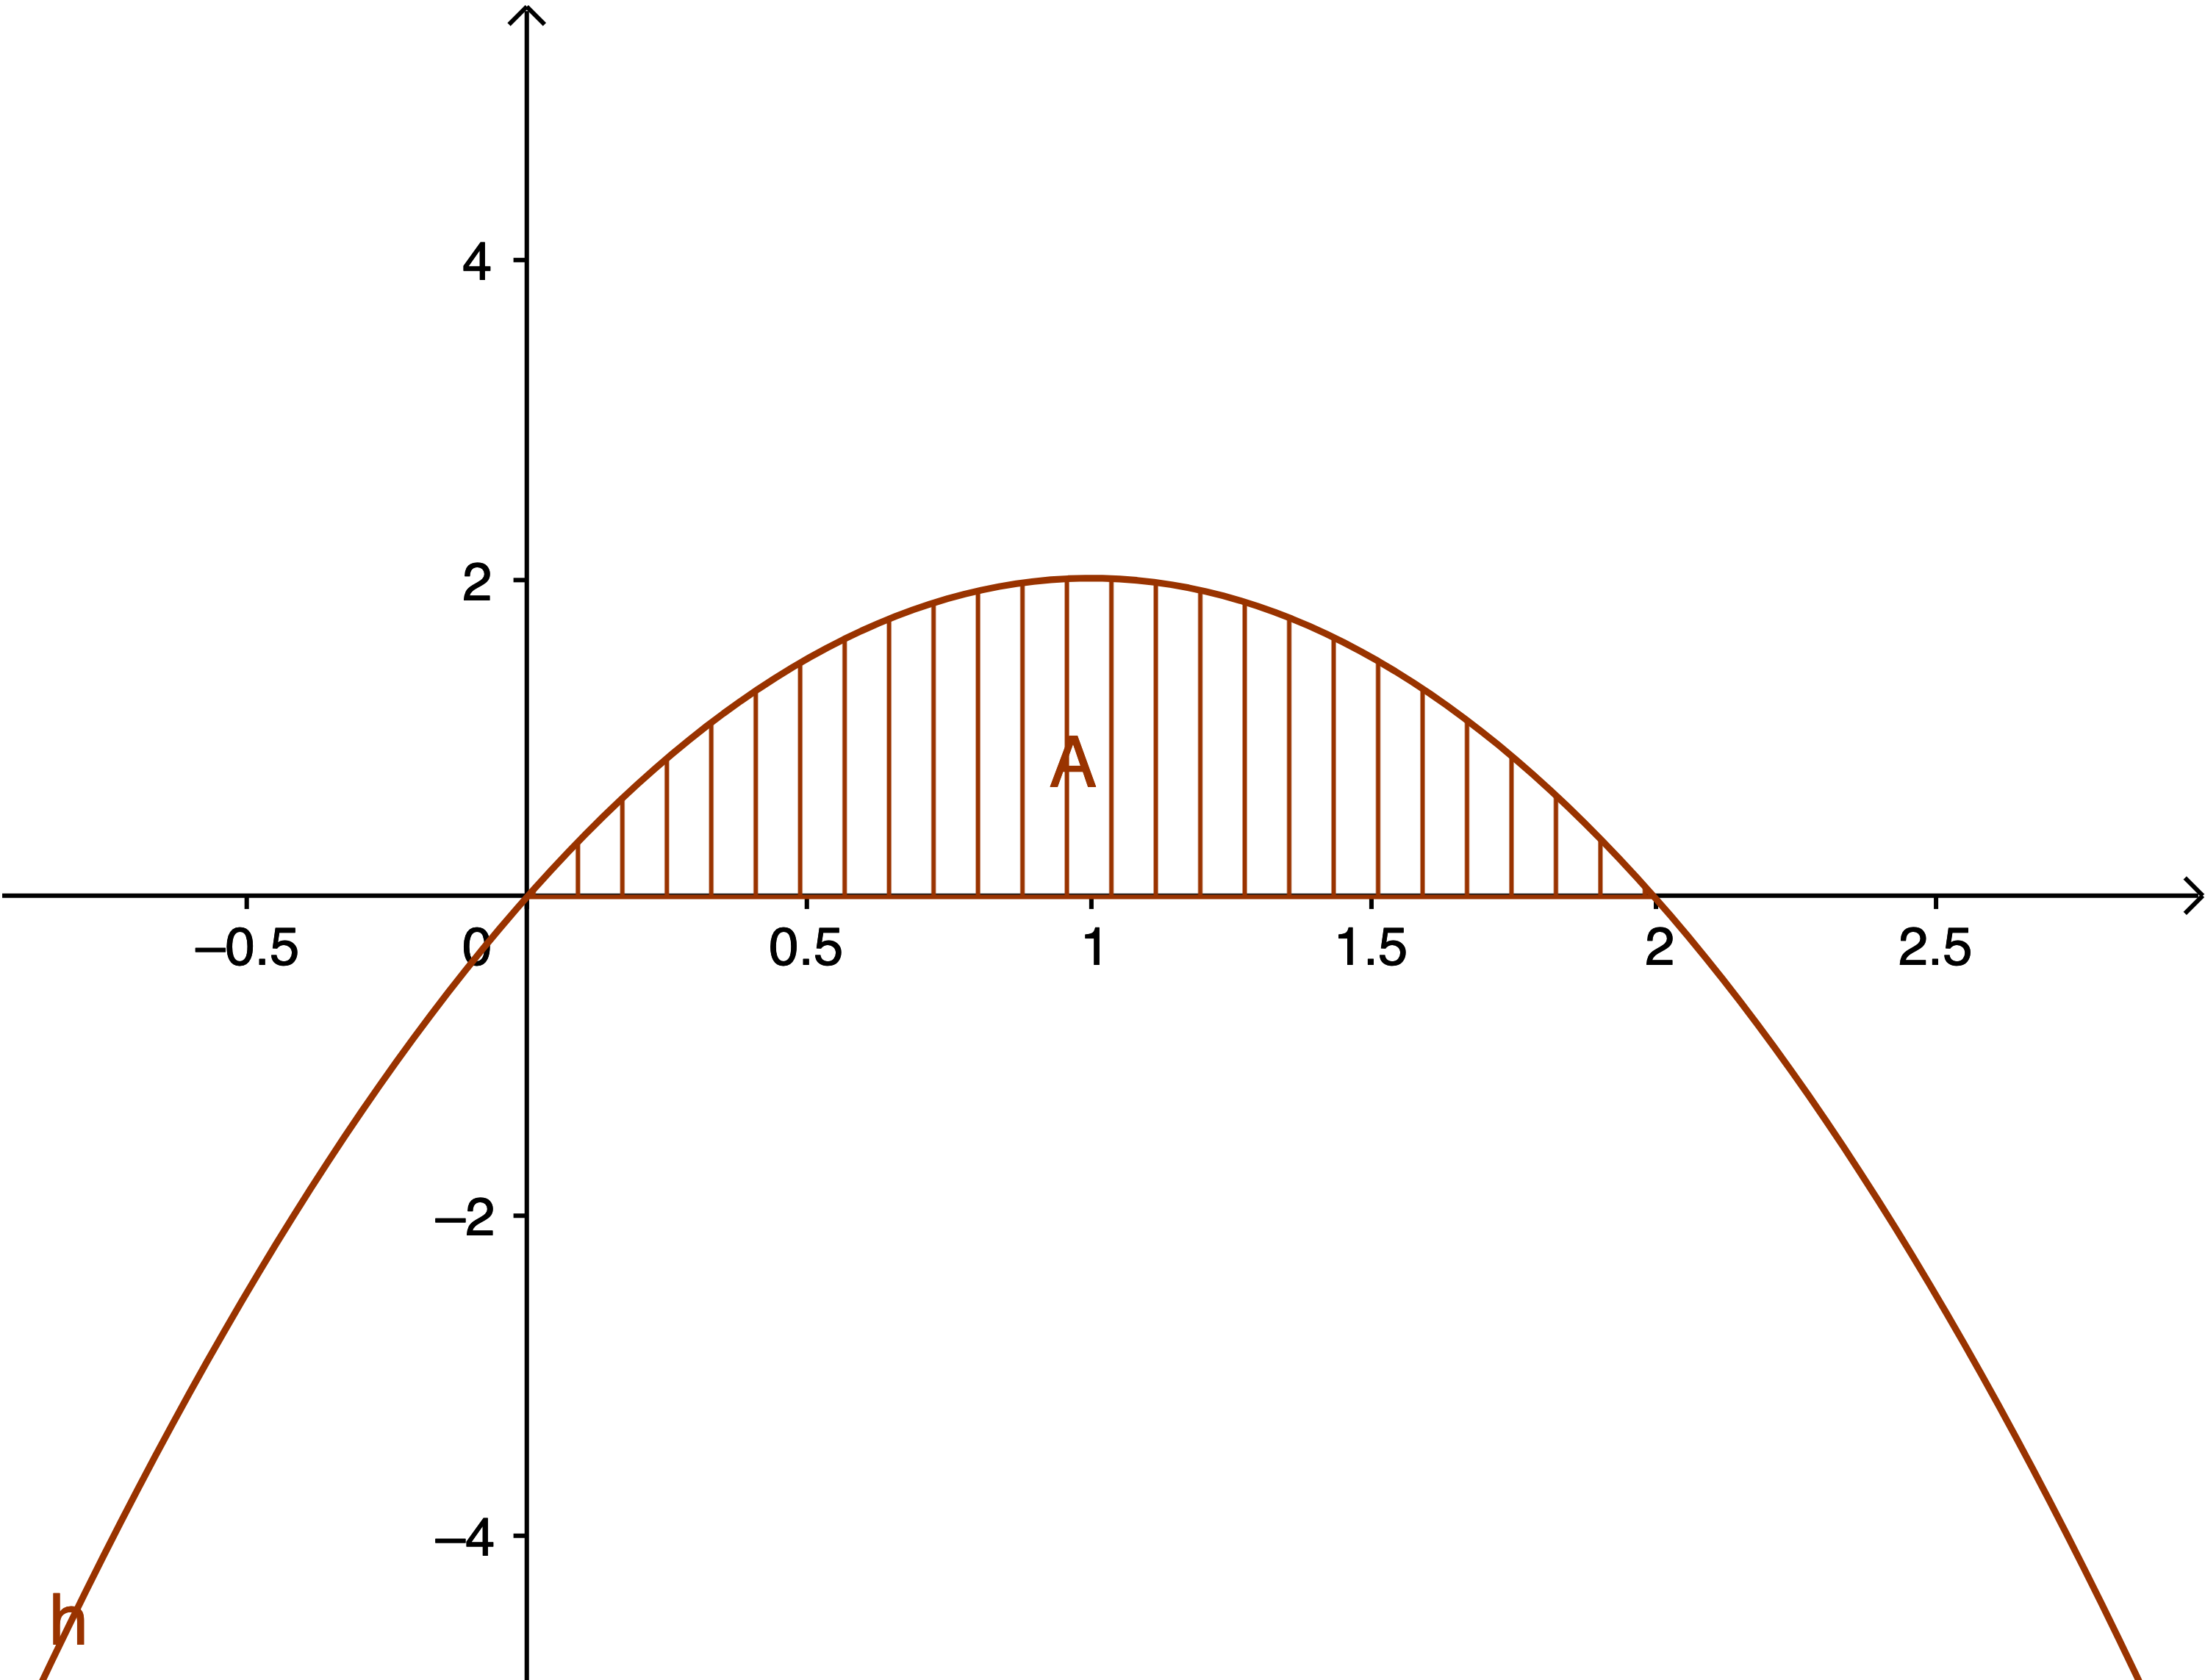
\includegraphics[width = 0.5\textwidth]{media/wal-tot.png}
	\end{center}
	Das ist der tote, gestrandete Wal. Die eingezeichneten Striche sind gleich lang, wie beim lebenden Wal. Die Funktion \(h\), ist demnach definiert durch
	\[ h(x)=g(x)-f(x)=-x^2+4x-2-(x^2-2)=-2x^2+4x \]
	Der Flächeninhalt ist unverändert und es gilt
	\[ A=\int_0^2 (g(x)-f(x))\, dx=\int_0^2 (-2x^2+4x) \, dx=\left[-\frac{2}{3} x^3+2x^2 \right]_0^2=-\frac{2}{3}\cdot 2^3+2\cdot 2^2-0=\frac{8}{3}  \]

\end{bsp}
\begin{satz}
	{Fläche zwischen zwei Graphen}{}

	Seien \(f\) und \(g\) zwei Funktionen, die sich an den Stellen \(x=a\) und \(x=b\) schneiden. Ferner sei \(f(x)\ge g(x)\) für alle \(x\in [a,b]\), das heisst, \(f\) ist die \glqq obere Funktion\grqq{}, \(g\) die \glqq untere Funktion\grqq{}. Dann gilt für den Inhalt der Fläche zwischen den beiden Graphen:
	\[ A=\int_a^b(f(x)-g(x))\, dx \]
	\begin{center}
		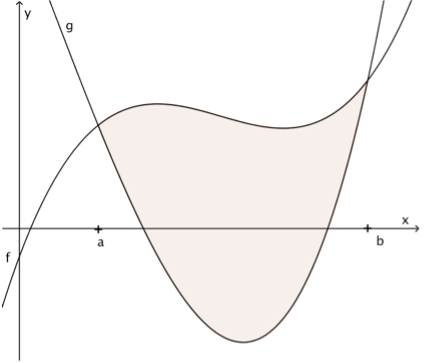
\includegraphics[width = 0.25\textwidth]{media/toterWalBild.png}
	\end{center}

\end{satz}
\begin{proof}
	Betrachten wir zunächst den Fall, wenn beide Kurven über der \(x\)-Achse verlaufen. Dann gilt:
	\begin{figure}[!htb]
		\centering
		\minipage{0.25\textwidth}
		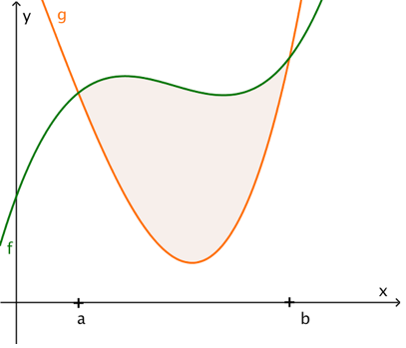
\includegraphics[width=\linewidth]{media/toterWalBew1.png}
		\endminipage \(=\)
		\minipage{0.25\textwidth}
		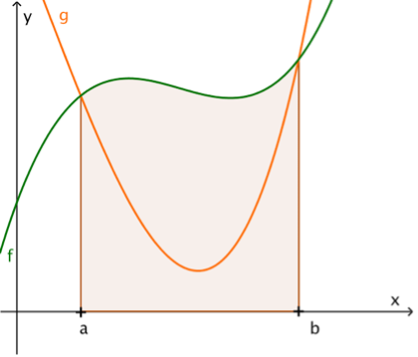
\includegraphics[width=\linewidth]{media/toterWalBew2.png}
		\endminipage \(-\)
		\minipage{0.25\textwidth}
		\includegraphics[width=\linewidth]{media/toterWalBew3.png}
		\endminipage
	\end{figure}

	In Formeln:
	\[ A=\int_a^b f(x)  \, dx -\int_a^b g(x)  \, dx = \int_a^b (f(x)-g(x)) \,dx \]
	Falls die Graphen teilweise oder ganz unter der \(x\)-Achse liegen, können sie zuerst durch Addition einer entsprechenden Konstante über die \(x\)-Achse verschoben werden. Bei der Differenz \(f(x)-g(x)\) fällt die Konstante wieder raus.

\end{proof}

\clearpage
\begin{bsp}
	{}{}
	Gegeben sind die Funktionen \(f(x)=2x^3-2x^2-4x\) und \(g(x)=-x^3+x^2+2x\). Gesucht ist der Flächeninhalt des endlichen Gebietes, welches durch die beiden Graphen eingeschlossen wird.
	\vspace{20cm}
\end{bsp}
\clearpage
\begin{ueb}
	{Polynomfunktionen}{}
	\begin{enumerate}
		\item Berechnen Sie den Inhalt des Flächenstückes, das die Graphen der Funktionen \(f_1\) und \(f_2\) einschliessen.
		      \begin{enumerate}
			      \item \(f_1: y=x,\qquad f_2: y=x^2\)
			      \item \(f_1: y=x,\qquad f_2: y=x^3\)
			      \item \(f_1: y=2x-3,\qquad f_2: y=x^2-2x-8\)
			      \item \(f_1: y=x^3,\qquad f_2: y=2x-x^2\)
			      \item \(f_1: y=x^2-3x,\qquad f_2: y=x^3-6x^2+9x\)
		      \end{enumerate}
		\item Welchen Inhalt hat das Flächenstück, das zwischen der Parabel \(y=3x-x^2\) und den Tangenten in den beiden Nullstellen der Parabel eingeschlossen wird?
		\item Berechnen Sie den Inhalt der Fläche zwischen dem Graphen \(f(x)= 3x(x^2-3x+2)\) und der Tangenten im Wendepunkt des Graphen und der \(y\)-Achse.
		\item Für welchen Wert von \(a\) schliessen die beiden Graphen der Funktionen \(f(x)=x^2-ax\) und \(g(x)= ax\) eine Fläche mit dem Inhalt \(A=36\) ein?
	\end{enumerate}
\end{ueb}
\begin{ueb}
	{Andere Funktionstypen}{}
	\begin{enumerate}\setcounter{enumi}{4}
		\item Berechnen Sie den Inhalt des Flächenstückes, das die Graphen der Funktionen \(f(x) = 2\sqrt{4-x}\) und \(g(x)=x^2-5x+4\) einschliessen.

		\item Berechnen Sie den Inhalt einer der (unendlich vielen) Flächenstücke, die zwischen der Graphen \(f(x)=\sin(x)\) und \(g(x)=1-\sin(x)\) liegen.
		\item Berechnen Sie den Inhalt einer der (unendlich vielen) Flächenstücke, die zwischen der Graphen \(f(x)=\sin(x)\) und \(g(x)=\sqrt{3}\cos(x)\) liegen.
		\item Berechnen Sie den Inhalt der Fläche zwischen den Graphen von \(f(x)=\frac{1}{x}\) und \(g(x) = \frac{2}{x}\) im Intervall \(x\in [1, 3]\).
	\end{enumerate}
\end{ueb}

\clearpage

\emph{Lösungen:}
\begin{enumerate}
	\item Flächen zwischen Polynomfunktionen:
	      \begin{enumerate}
		      \item \(A=\frac{1}{6}\)
		      \item \(A=\frac{1}{2}\)
		      \item \(A= 36\)
		      \item \(A= \frac{37}{12}\)
		      \item \(A=11.83\bar{3}\)
	      \end{enumerate}
	\item \(A=2.25\)
	\item \(A=\frac{3}{4}\)
	\item \(a=\pm3\)
	\item \(A=13.33\bar{3}\)
	\item Schnittstellen: \(x_1= \frac{\pi}{6}\), \(x_2= \frac{5\pi}{6}\), Flächeninhalt \(A=2\sqrt{3}-\frac{2\pi}{3}\)
	\item Schnittstellen: \(x_1= \frac{\pi}{3}\), \(x_2= \frac{4\pi}{3}\), Flächeninhalt \(A=4\)
	\item \(A= \ln(3)\)
\end{enumerate}









































\clearpage
\subsubsection{Volumen}
\begin{LA}
	{Das Volumen der Pyramide}{}
	Wie sie wissen, lautet die Formel zur Berechnung des Volumens einer Pyramide \(V=\frac{1}{3} Gh\). Diese Formel wurde zwar schon etwa 400 v.Chr. von Demokrit entdeckt, der Beweis für ihre Richtigkeit ist aber nicht einfach. Eine Methode, welche schon im Altertum angewendet wurde, besteht darin, die Pyramide durch einen Stapel dünner, quaderförmigen Scheiben anzunähern.
	\begin{center}
		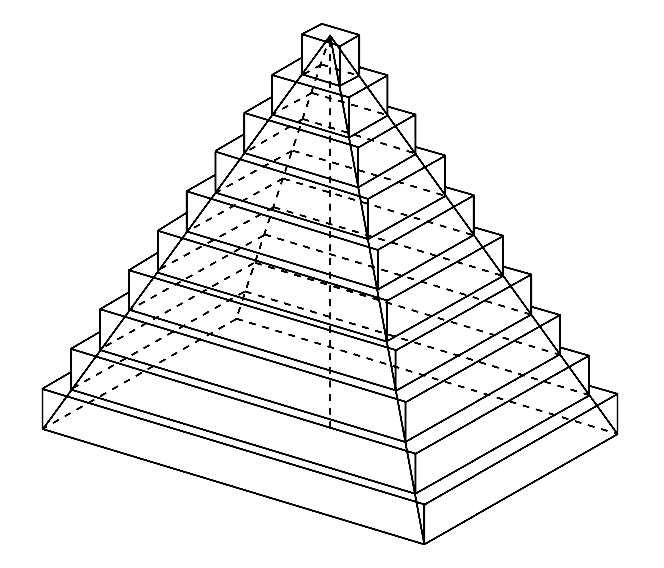
\includegraphics[width = 0.5\textwidth]{media/pyramideInScheiben.png}
	\end{center}

	Der Einfachheit halber betrachten wir eine gerade, vierseitige Pyramide. Damit wir die Volumina der einzelnen Quader im Bild oben berechnen können, benötigen wir eine Formel für den Flächeninhalt \(A(x)\) einer parallel zur Grundfläche liegenden Schnittfläche durch die Pyramide im Abstand \(x\) von der Spitze der Pyramide.
	\begin{center}
		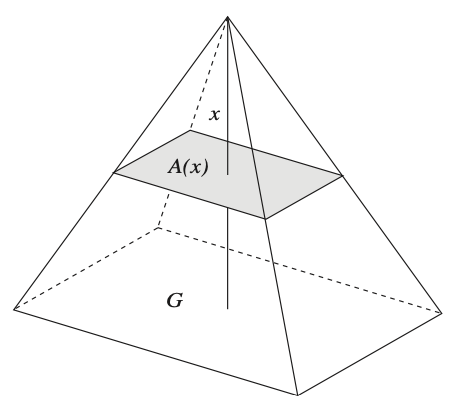
\includegraphics[width = 0.5\textwidth]{media/pyramideMitQuerschnit.png}
	\end{center}
	Die Pyramide mit der Grundfläche \(G\) und der Höhe \(h\) ist ähnlich zu jener mit Grundfläche \(A(x)\) und Höhe \(h\). Daraus ergibt sich:
	\[\frac{A(x)}{G} = \left(\frac{x}{h}\right)^2 \Longrightarrow A(x)=\frac{G}{h^2}\cdot x^2 \]

	\begin{enumerate}
		\item 	Angenommen die Pyramide wird durch vier Quadern angenähert. Wie lautet dann das approximative Volumen in Abhängigkeit von \(G\) und \(h\)?
		      (Kontrolle: \(V\approx \frac{15}{32} Gh\) )
		\item Die in der Skizze verwendeten Quader sind alle ein wenig zu gross. Wie lautet eine entsprechende Annäherung durch 4 Quadern, die alle im Inneren der Pyramide liegen und damit ein wenig zu klein sind? (Beachten Sie, dass der oberste der vier Quader dann das Volumen 0 hat.)
		      (Kontrolle: \(V\approx \frac{7}{32} Gh\) )
		\item Betrachten Sie nun den Graphen der Funktion \(A(x)=\frac{G}{h^2}\cdot x^2\) im Intervall \([0,h]\) (unten) und berechnen Sie den Wert der Untersumme \(U_4\).
		      \begin{center}
			      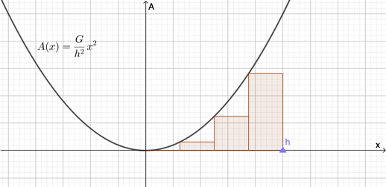
\includegraphics[width = 0.5\textwidth]{media/graphZurPyramide.png}
		      \end{center}
		\item Vergleichen Sie Ihre Rechnungen für die Aufgaben 2. und 3. Was stellen Sie fest? Was folgt daraus für die Berechnung des exakten Volumens einer Pyramide.
	\end{enumerate}

\end{LA}
\clearpage
Mit bestimmten Integralen können nicht bloss Flächeninhalte berechnet werden, sondern auch Volumina von Körpern:
\begin{satz}
	{Merksatz}{}
	Das Volumen eines Körpers ist das Integral über die Querschnittsfläche.
	\begin{center}
		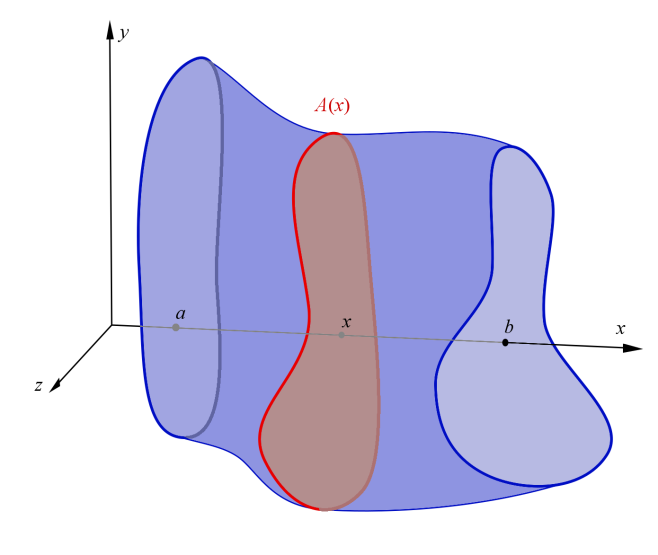
\includegraphics[width = 0.5\textwidth]{media/querschnitt.png}
	\end{center}
	\[ V = \int_a^b A(x) \, dx\]
\end{satz}
Besonders einfach ist damit die Berechnung von Volumina von Körpern, die durch Rotation eines Graphen um die \(x\)-Achse entstehen. Das folgende Beispiel soll dies veranschaulichen.
\begin{bsp}
	{Rotationsvolumen}{}
	Betrachten Sie die Kurve \(y=\sqrt x\) im Intervall \(x\in[0,1]\). Wird diese Kurve um die \(x\)-Achse gedreht, so entsteht ein sogenanntes Paraboloid:
	\begin{center}
		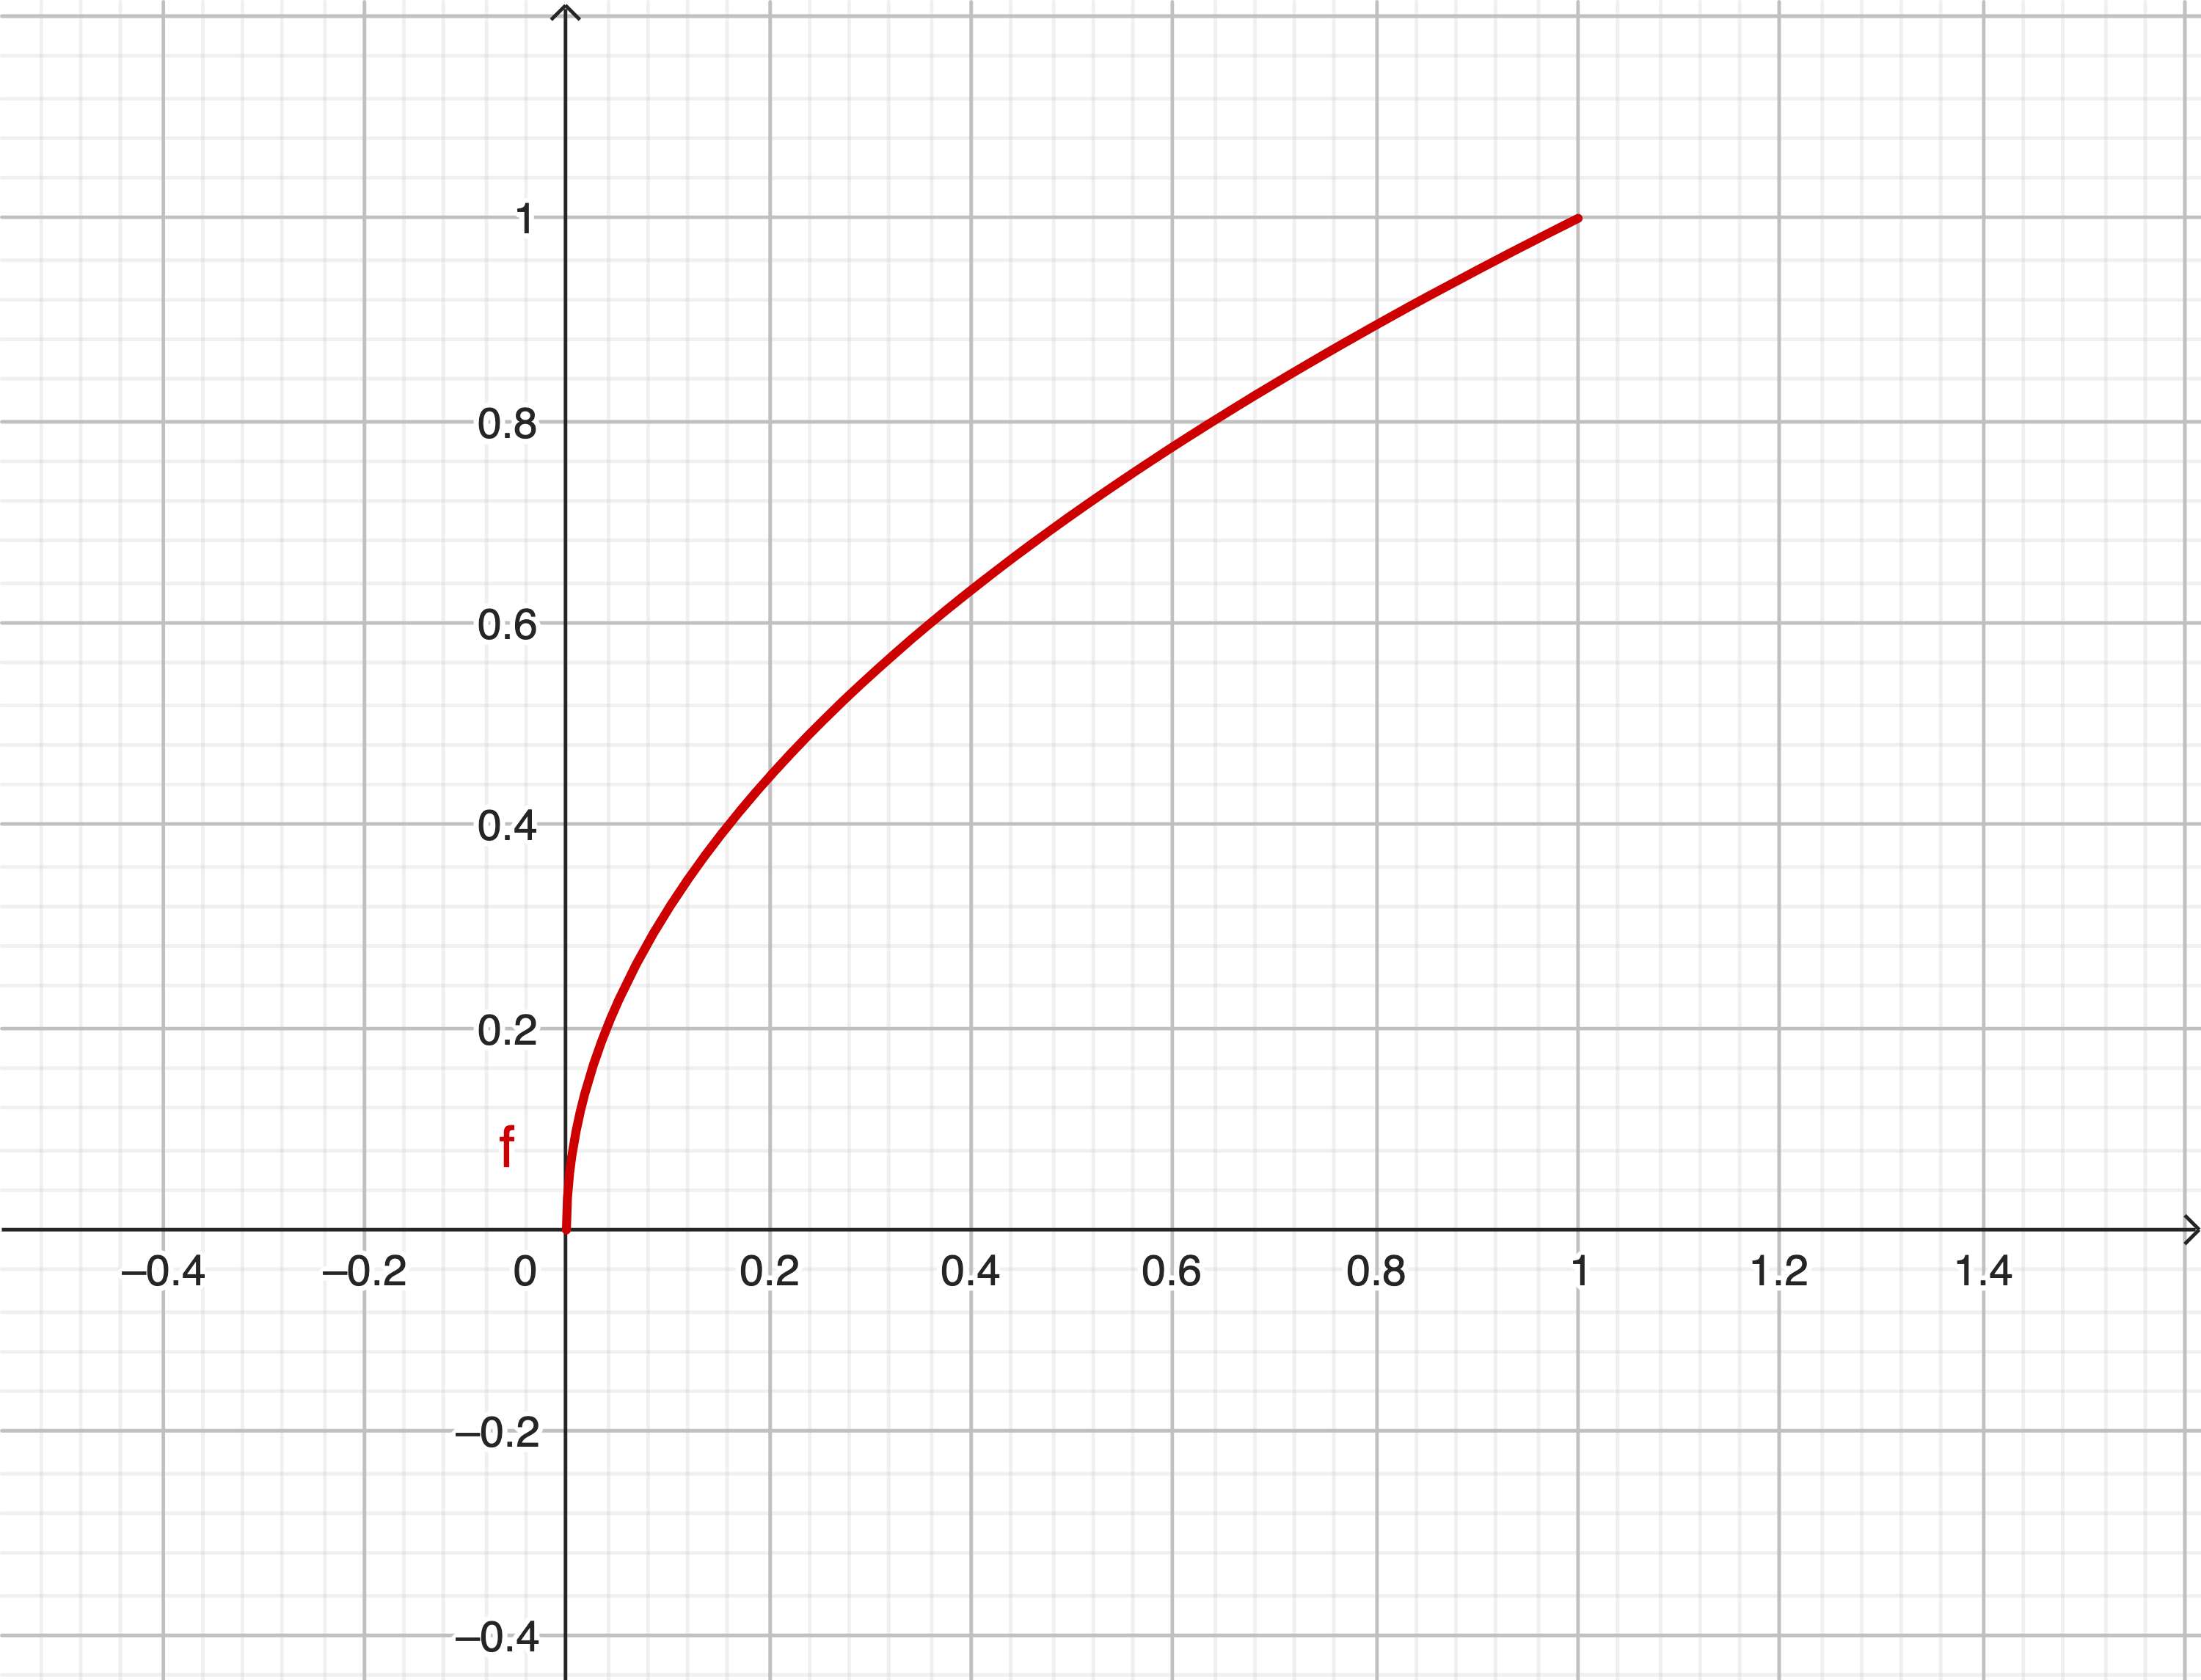
\includegraphics[width = 0.4\textwidth]{media/IntroRotationsVolumen2dv2.png}\hfill
		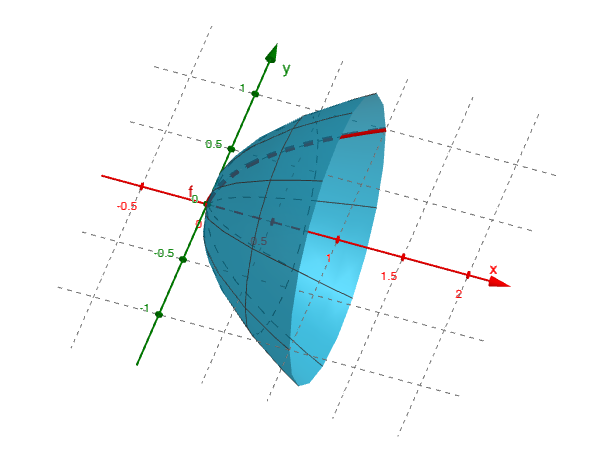
\includegraphics[width = 0.4\textwidth]{media/IntroRotationsVolumen3dv2.png}
	\end{center}

	% \begin{figure}[!htb]
	%     \minipage{0.4\textwidth}
	%       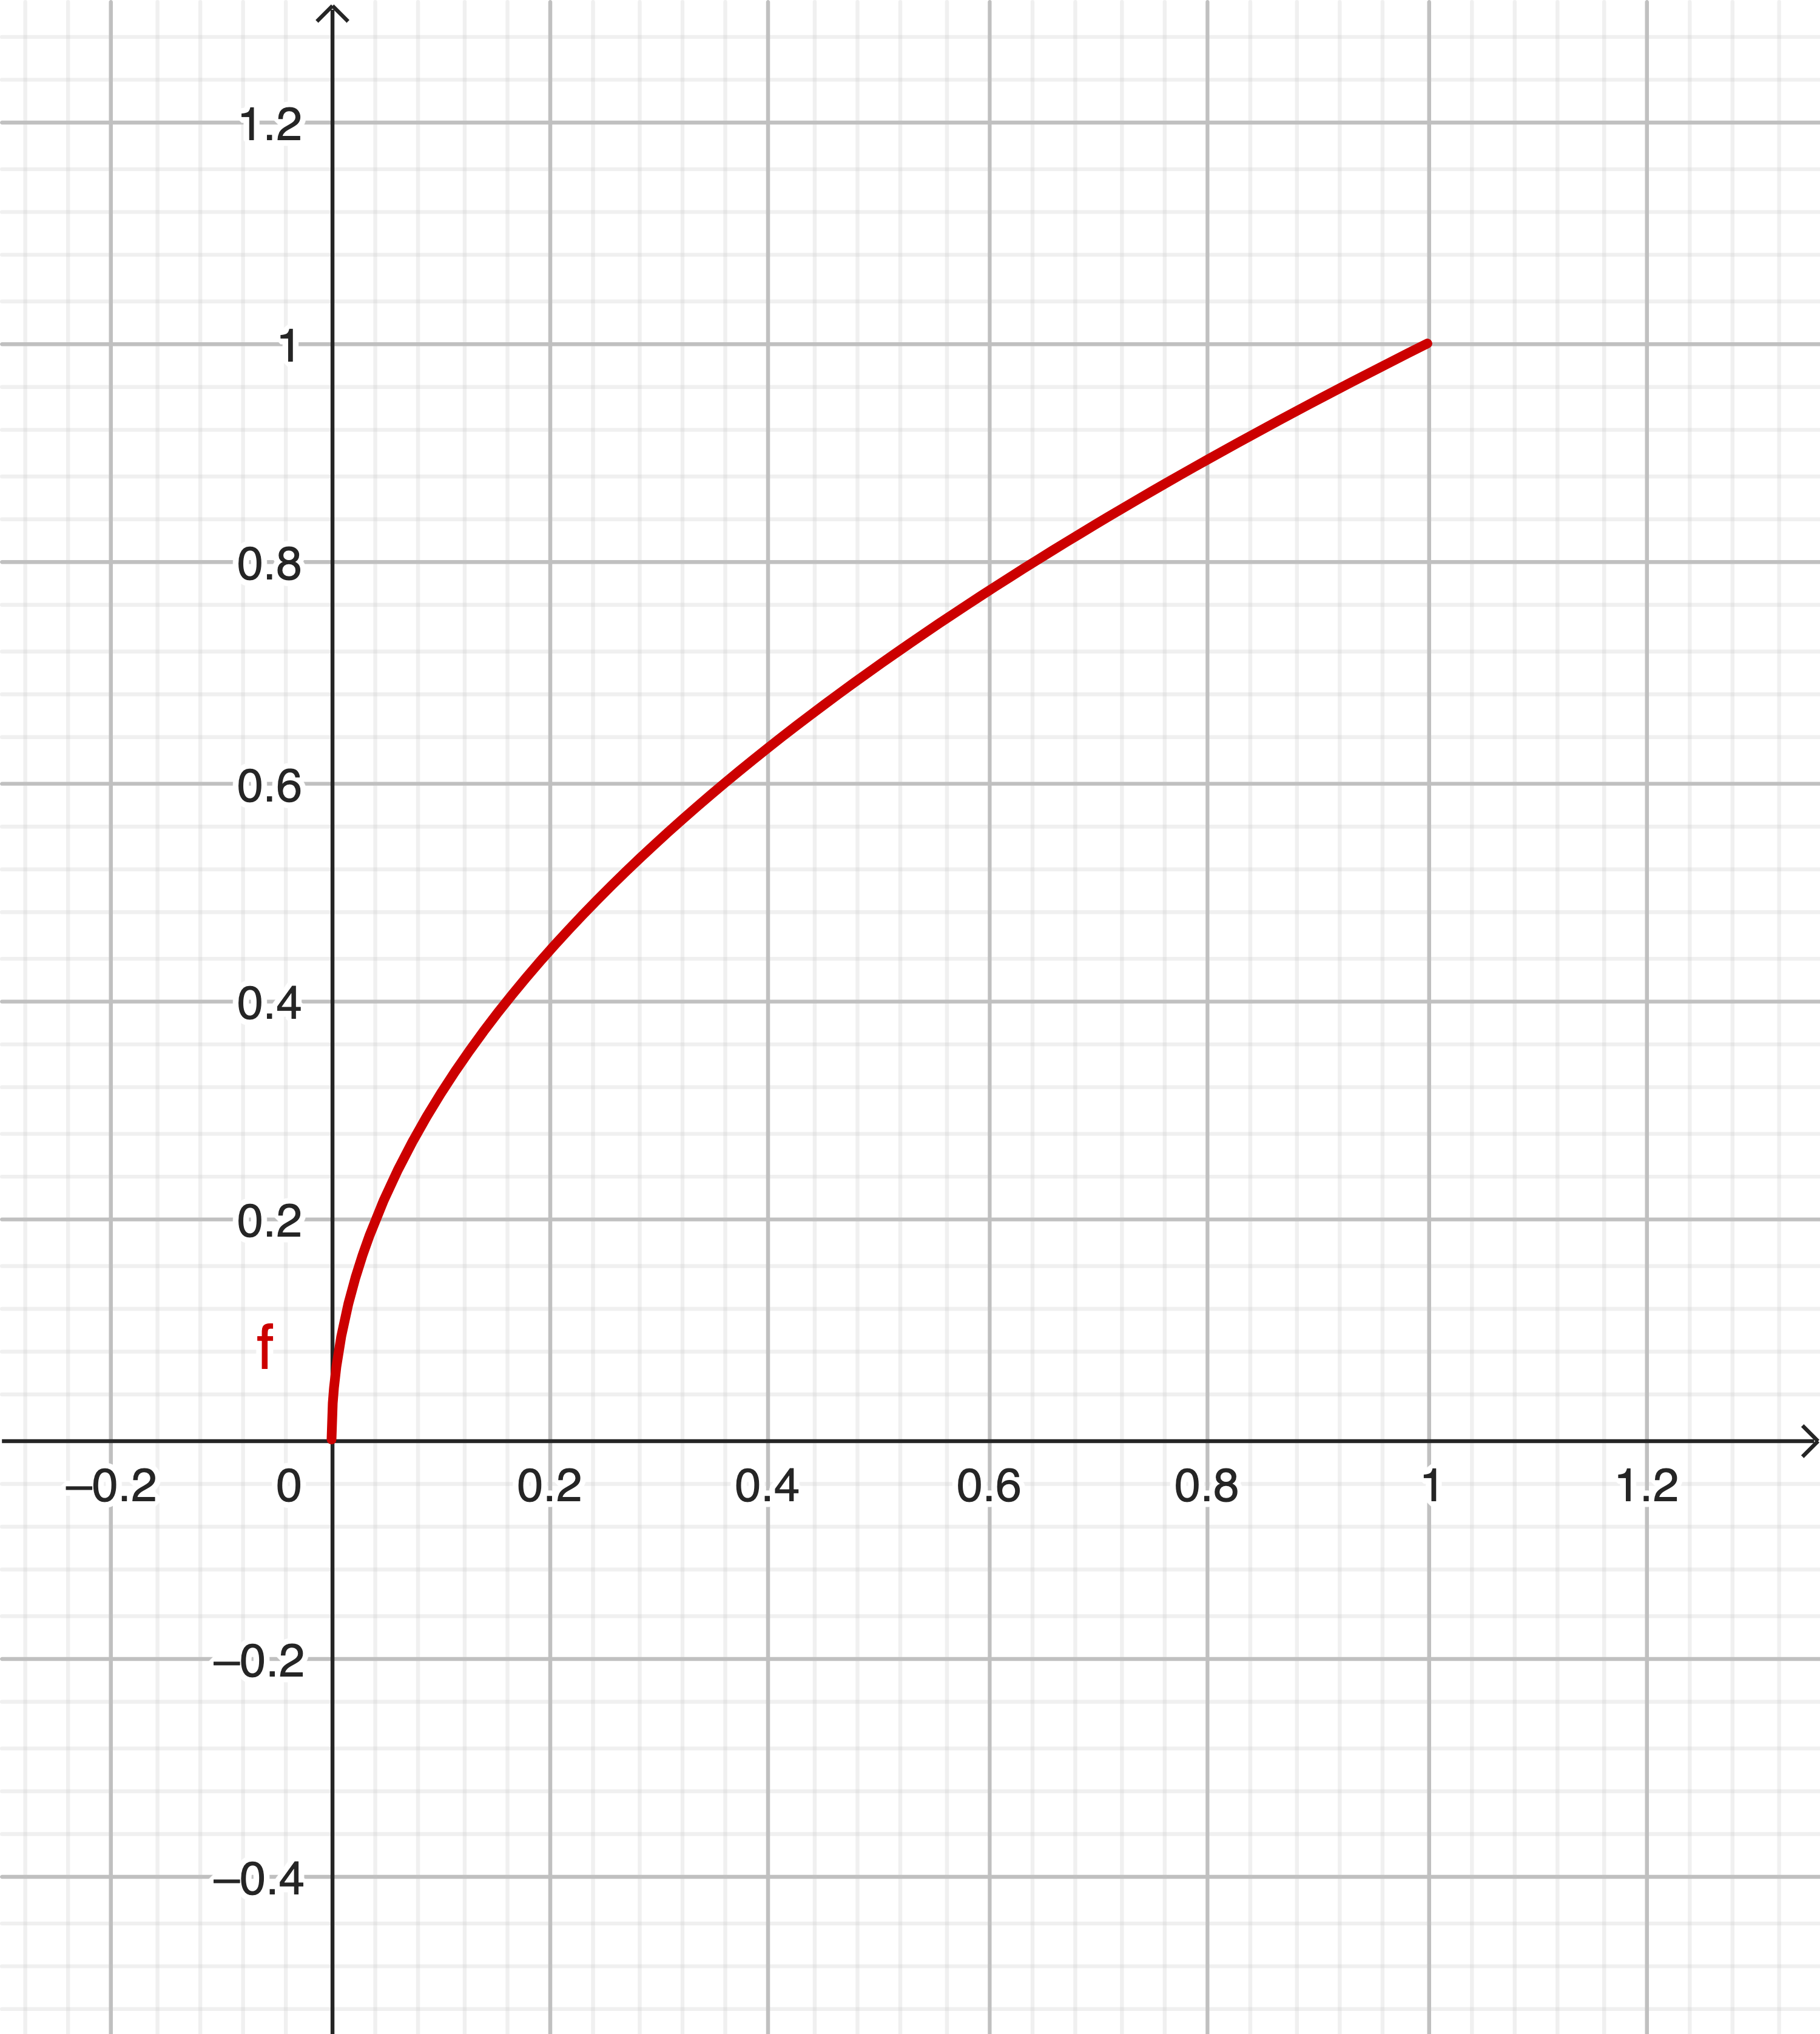
\includegraphics[width=\linewidth]{media/IntroRotationsVolumen2D.png}
	%     \endminipage\hfill
	%     \minipage{0.4\textwidth}
	%       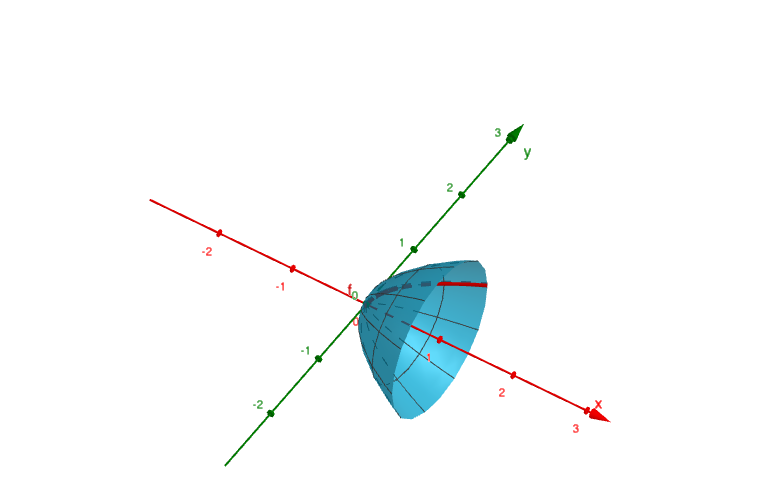
\includegraphics[width=\linewidth]{media/IntroRotationsVolumen3D.png}
	%     \endminipage
	% \end{figure}

	Die Querschnittsflächen des Paraboloids, die senkrecht zur \(x\)-Achse stehen, sind Kreise mit dem Radius \(y=\sqrt x\). Der Flächeninhalt dieser Kreise ist demnach \(A(x)=\pi y^2=\pi (\sqrt x)^2=\pi x\). Das Volumen des Paraboloids beträgt damit
	\[V=\int_0^1 \pi y^2 \, dx =\int_0^1\pi x \, dx=\left[\frac{\pi}{2} x^2 \right]_0^1= \frac{\pi}{2}\cdot 1^2-\frac{\pi}{2}\cdot 0^2=\frac{\pi}{2}\]

\end{bsp}
Allgemein gilt:
\begin{satz}
	{Rotationsvolumen}{}
	Wird eine Kurve \(y=f(x)\) im Intervall \([a,b]\) um die \(x\)-Achse gedreht, entsteht ein Körper mit dem Volumen
	\[V=\int_a^b \pi \cdot (f(x))^2 dx\]

\end{satz}


\textbf{Bemerkung}: Da \(\pi\) ein konstanter Faktor ist, kann man ihn auch vor das Integral stellen.
\[V=\pi \cdot\int_a^b  (f(x))^2 dx\]

\begin{bsp}{}{}
	Die endliche Fläche zwischen der \(x\)-Achse und der Kurve \(y=4-x^2\) rotiert um die \(x\)-Achse. Bestimmen Sie das Volumen des Rotationskörpers?
	\begin{center}
		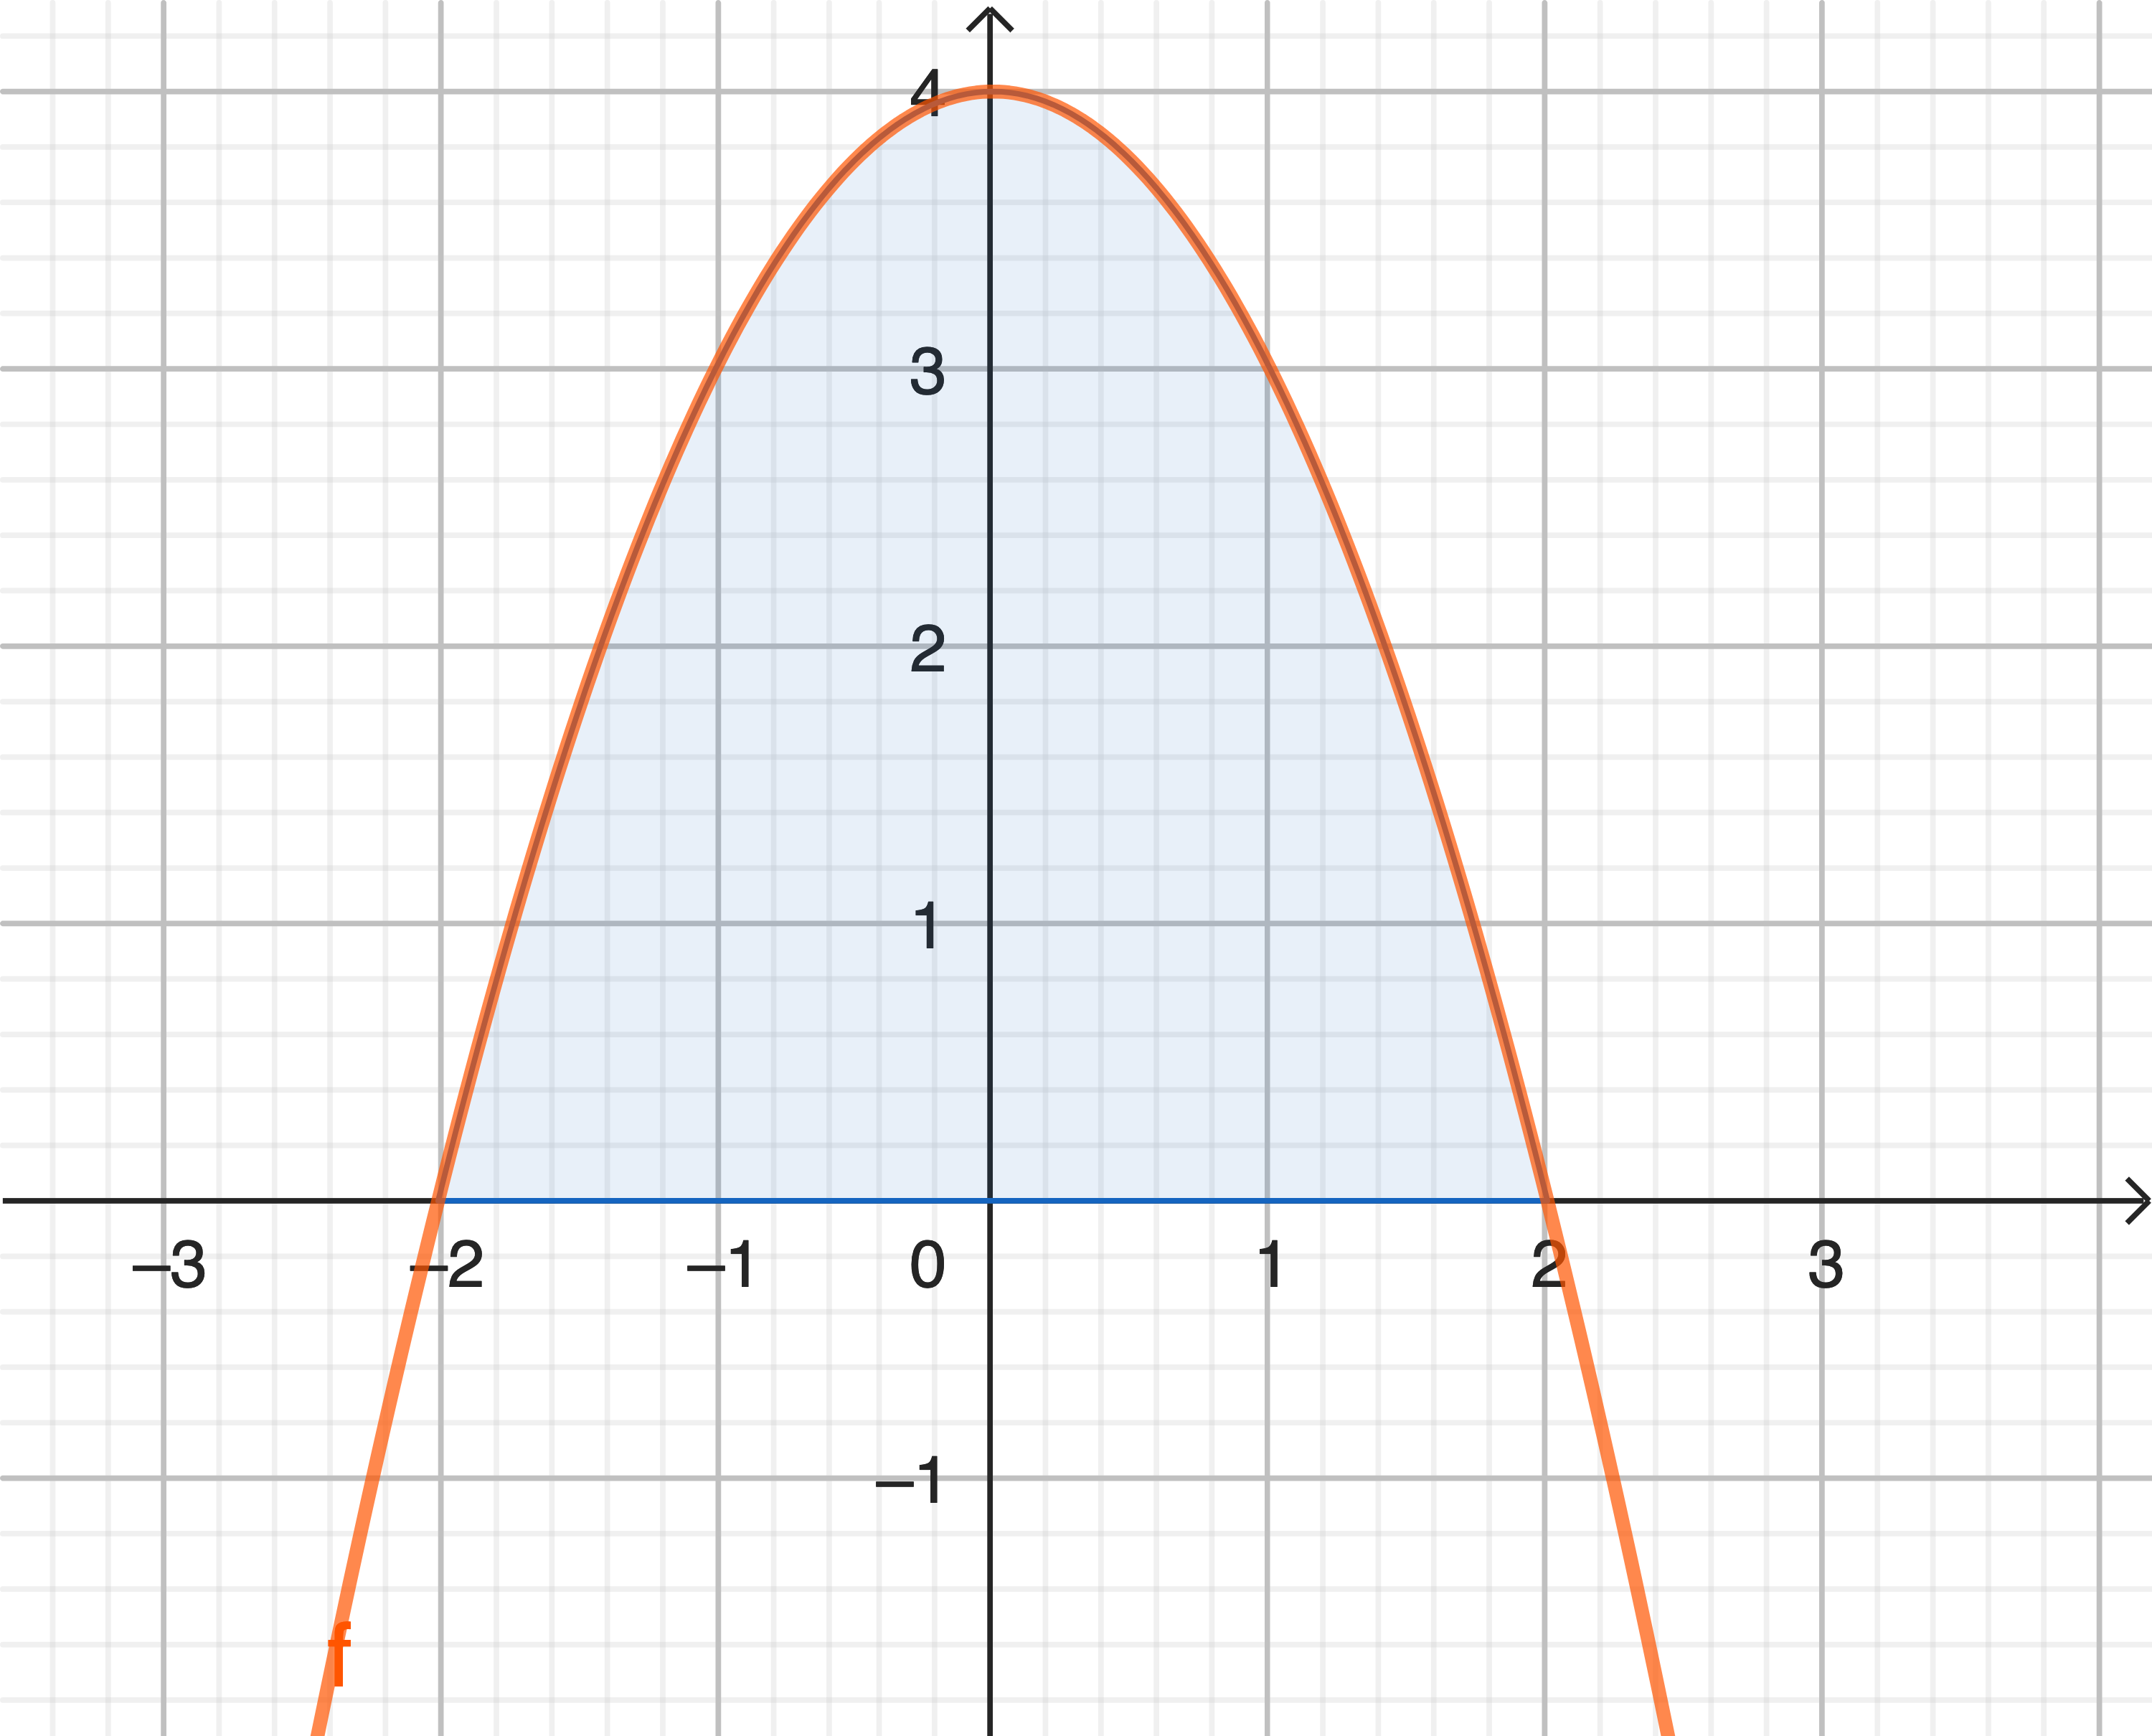
\includegraphics[width = 0.5\textwidth]{media/rotationsVolumenBsp2.png}
	\end{center}

	\vspace*{6cm}
	% Die Fläche zwischen Kurve und $x$-Achse wird durch die Nullstellen der Kurve begrenzt. Diese sind:
	% $$4-x^2=0 \iff 4=x^2 \iff x_{1,2}=\pm 2$$
	% Damit gilt für das Volumen des Rotationskörpers
	% $$ V=\pi \cdot \int_{-2}^2 (4-x^2)^2 \, dx =\pi \cdot \int_{-2}^2 (16-8x^2+x^4 )  \, dx =\pi \cdot \left[16x-\frac{8}{3} x^3+\frac{1}{5} x^5 \right]_{-2}^2=\frac{160}{3} \pi $$ 

\end{bsp}

\clearpage
\begin{ueb}
	{}{}
	\begin{enumerate}
		\item Die endliche Fläche zwischen der gegeben Kurve und der \(x\)-Achse rotiert um die \(x\)-Achse. Berechnen Sie das Volumen der Rotationskörpers.
		      \begin{enumerate}
			      \item \(y=2x-x^2\)
			      \item \(y=x^3-3x^2\)
			      \item \(y=\sqrt{1-x^2}\)
		      \end{enumerate}
		\item Die Fläche zwischen den beiden Kurven rotiert um die \(x\)-Achse. Berechnen Sie das Volumen des Rotationskörpers.
		      \begin{enumerate}
			      \item \(y=x\) und \(y=x^3\)
			      \item \(y=x^2+3\) und \(y=-2x^2+6\)
		      \end{enumerate}
		\item Die Kurve \(y=\frac{1}{4}x^3\) und die Kurventangente im Punkt \(P=(2, y_P)\) begrenzen im 1. Quadranten eine Fläche, die um die \(x\)-Achse rotiert wird. Berechnen Sie das Volumen des Rotationskörpers.
		\item Challenge: Perlenkette
		      \begin{enumerate}
			      \item Zeigen Sie, dass \(F(x)=\frac{1}{2}\left(x-\sin(x) \cdot \cos(x)\right)\) eine Stammfunktion der Funktion \(f(x) = \sin^2(x)\) ist. Benutzen Sie dazu den trigonometrischen Pythagoras.
			      \item   Wenn die Sinuskurve um die \(x\)-Achse rotiert, ensteht eine Art unendliche Perlenkette. Berechnen Sie das Volumen eines der Glieder dier Kette.
		      \end{enumerate}

	\end{enumerate}


\end{ueb}

\clearpage
\emph{Lösungen:}
\begin{enumerate}
	\item Rotationsvolumen:
	      \begin{enumerate}
		      \item \(V=\frac{16}{15}\pi\)
		      \item \(V=\frac{729}{35}\pi\)
		      \item \(V=\frac{4}{3}\pi\) (Der Körper ist eine Kugel mit Radius 1!)
	      \end{enumerate}
	\item Rotationsvolumen zwischen zwei Kurven:
	      \begin{enumerate}
		      \item \(V=\frac{8}{21}\pi\)
		      \item \(V\approx 110.58\)
	      \end{enumerate}
	\item \(V=\frac{16}{63}\pi\)
	\item Perlenkette:
	      \begin{enumerate}
		      \item Mit der Produktregel ableiten und mit dem trigonometrischen Pythagoras \(1-\cos^2(x)=\sin^2(x)\) vereinfachen.
		      \item \(V=\frac{\pi^2}{2}\)
	      \end{enumerate}

\end{enumerate}

\clearpage
\subsubsection*{Volumen als Integral der Querschnittsfläche}
In diesem Abschnitt werden Sie Volumen von Körpern berechnen, die nicht aus der Rotation um eine Achse entstanden sind. Diese Volumina können als Integrale der entsprechenden Querschnittsflächen berechnet werden:
\[ V= \int_{a}^{b} A(x) dx\]

\begin{ueb}
	{Das Volumen der Quarterpipe}{quarterpipe}
	Um das Volumen einer Quarterpipe zu berechnen, wird diese in ein Koordinatensystem eingebettet. Dabei modellieren wir die Quarterpipe als einen Körper, der dadurch ensteht, dass man die Parabel \(y=\frac{1}{20} x^2\) senkrecht zur \(xy\)-Ebene verschiebt. Den Körper approximieren wir durch dünne Quader, deren Grundfläche Querschnitte der Quarterpipe sind.
	\begin{center}
		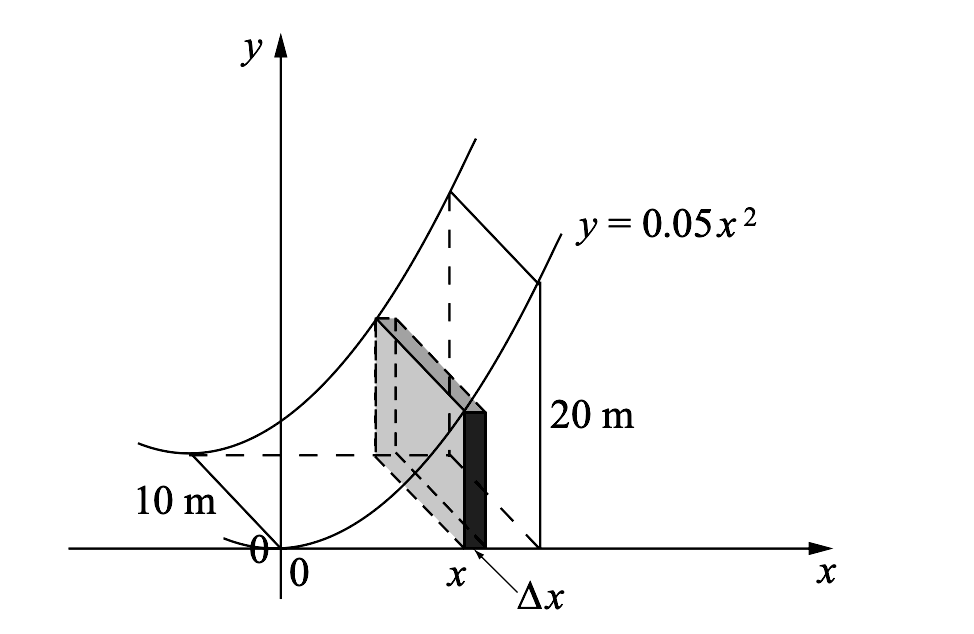
\includegraphics[width = 0.5 \textwidth]{media/quarterpipe.png}
	\end{center}
	\begin{enumerate}
		\item Berechnen Sie den Flächeninhalt \(A(x)\) eines Querschnitts der Quarterpipe im Abstand \(x\) vom Ursprung.
		\item Berechnen Sie das Volumen der Quarterpipe, indem Sie die Querschnittsfläche integrieren. Beachten Sie, dass Sie zuerst die obere Grenze des Integrals ermitteln müssen.
		\item Das Volumen könnte man auch wie bei einem Prisma mit \(V = G \cdot h\) berechnen. Prüfen Sie, ob die beiden Resultate übereinstimmen.
	\end{enumerate}
\end{ueb}

\begin{ueb}
	{Keil aus Baumstamm}{keil}
	Aus einem zylindrischen Baumstamm wird durch zwei ebene Schnitte ein Keil herausgeschlagen. Der Baumstamm habe einen Durchmesser von \(\SI{40}{\centi\metre}\). Die eine Schnittebene ist senkrecht zur Zylinderachse und die andere ist gegenüber dieser Ebene um \(30^\circ\) geneigt. Beide Ebenen schneiden sich längs eines Kreisdurchmessers.
	\begin{center}
		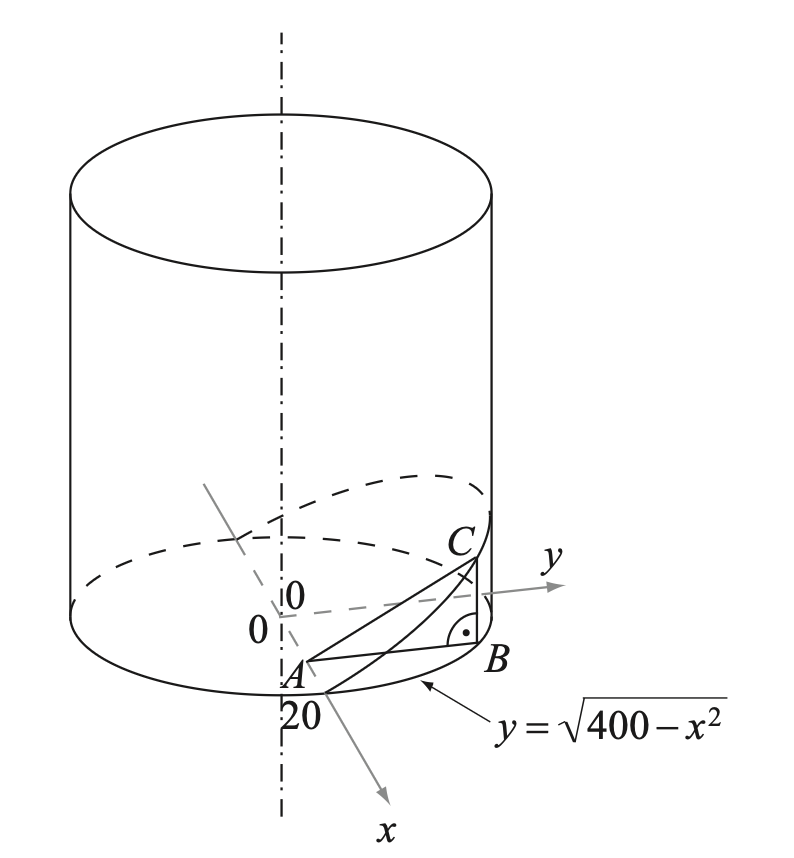
\includegraphics[width = 0.5 \textwidth]{media/keilBaumstamm.png}
	\end{center}

	Berechnen Sie das Volumen des herausgeschnittenen Keils.
\end{ueb}

%% Benötigt so partielle Integraion
% \begin{ueb}
%     {Tarp}{tarp}
%     Betrachten Sie die Abbildung. Eine Gerade in der \(xy\)-Ebene ist durch die Gleichung
%     \[
%         y = g(x) = 1-x
%     \]
%     gegeben. Sie schneidet die \(x\)-Achse in \(A\) und die \(y\)-Achse in \(B\). In der \(xz\)-Ebene ist der Graph der Funktion
%     \[
%         z = f(x) = e^{-x}
%     \]
%     gegeben. Er schneidet die \(z\)-Achse in \(C\).

%     Punkt \(D\) hat die gleiche \(x\)-Koordinate wie \(A\) und liegt auf dem Graphen von \(f\). Die Punkte auf den Graphen von \(g\) und \(f\) werden durch Strecken parallel zur \(yz\)-Ebene verbunden. Dadurch entsteht eine gekrümmte Fläche \(ABCD\).

%     Berechnen Sie das Volumen des Körpers, der durch die Fläche \(ABCD\) und die drei Koordinatenebenen begrenzt wird.
%     \begin{center}
%         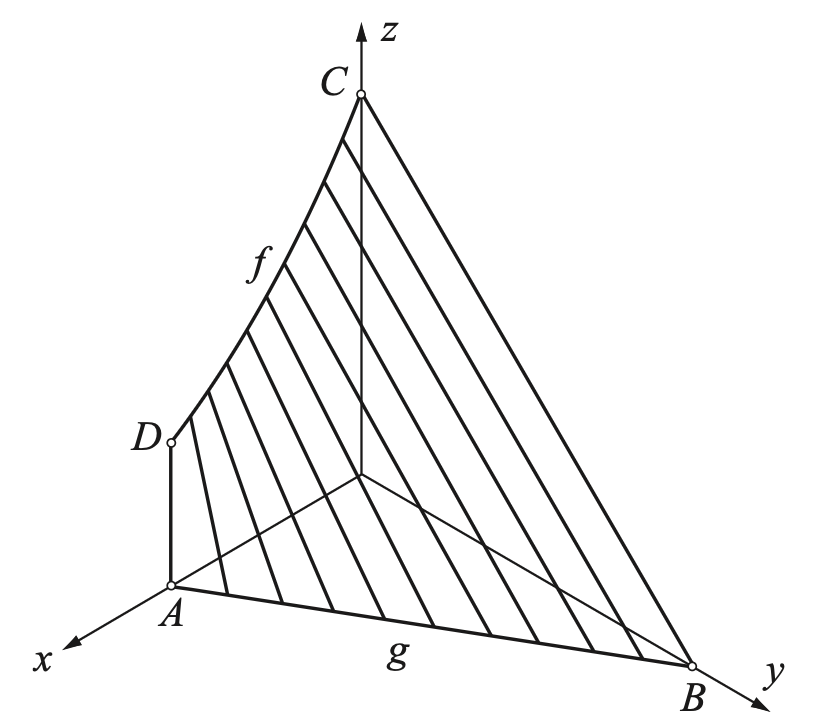
\includegraphics[width = 0.5 \textwidth]{media/Tarp.png}
%     \end{center}

% \end{ueb}

\emph{Lösungen:}
\Cref{uebng:quarterpipe}:\newline

\begin{enumerate}
	\item Die Querschnittsfläche ergibt sich aus der Höhe
	      \[
		      y(x)=\frac{1}{20}x^2
	      \]
	      und der Breite 10 der Quarterpipe. Damit gilt
	      \[
		      A(x)= 10\cdot \frac{1}{20}x^2 = \frac{1}{2}x^2
	      \]

	\item Die maximale Höhe der Pipe ist \(y=20\). Damit kann man den entsprechenden \(x\)-Wert berechnen:
	      \[ 20 = \frac{1}{20}x^2 \Rightarrow x = 20\]
	      Das Volumen der Quarterpipe ist demnach:
	      \[ V = \int_{0}^{20} A(x) dx = \int_0^{20} \frac{1}{2}x^2\,dx
		      =
		      \left[\frac{1}{6}x^3\right]_0^{20}
		      =
		      \frac{4000}{3}\]

	\item Alternativ kann der Körper als Prisma mit der Grundfläche unter der Parabel betrachtet werden:
	      \[
		      V = G\cdot h = \int_0^{20} \frac{1}{20} x^2 dx  \quad \cdot \quad 10 = \frac{400}{3} \cdot 10 =  \frac{4000}{3}
	      \]
	      Beide Berechnungen liefern dasselbe Resultat.
\end{enumerate}

\emph{Lösungen:}\Cref{uebng:keil}

Für einen Querschnitt im Abstand \(x\) vom Mittelpunkt gilt \(\overline{AB} = \sqrt{400-x^2}\) und \(\overline{BC} = \overline{AB} \cdot \tan(30^\circ)\). Damit folgt:
\[
	A(x)=\frac{1}{2}\sqrt{400-x^2} \cdot \sqrt{400-x^2}\tan(30^\circ) = \frac{\sqrt{3}}{6}\left(400-x^2\right)
\]
Damit
\[
	V=\int_{-20}^{20} A(x)\,dx
	=\frac{2}{3}r^3\tan(30^\circ)
	=\frac{16000}{3\sqrt{3}}\,\si{\centi\metre\cubed}
	\approx \SI{3079}{\centi\metre\cubed}
\]






% \clearpage
% \textbf{Mittelwert einer Funktion}
% \begin{LA}
%     {Der Mittelwert einer Funktion}{}
%     In Breitengraden wie jenem von Zürich kann die Tageslänge von Sonnenaufgang bis Sonnenuntergang grob durch die Funktion mit der Gleichung 
%     $$ T(x) = 4 \sin\left(\frac{2\pi}{365} (x-80)\right) +12 $$
%     angenähert werden, wobei $x$ die Nummer des Tages im Jahr und $T$ die Tageslänge in Stunden ist.
%     \begin{enumerate}
%         \item Zeichnen Sie den Graphen der Funktion mit Geogebra im Bereich $x\in[0, 365]$. An welchem Datum sind Tag und Nacht gleich lang? Wann ist der längste/kürzeste Tag?
%         \item Welches ist die mittlere Tageslänge über ein Jahr betrachtet?
%         \item Allgemein versteht man unter dem \emph{Mittelwert} einer positiven stetigen Funktion $y=f(x)$ im Intervall $x\in[a,b]$, jenen Wert $y_M$, bei dem der Flächeninhalt des Rechtecks mit der Höhe $y_M$ über dem Intervall $[a,b]$ gleich gross ist wie der Flächeninhalt des Gebietes zwischen dem Graphen von $f$ und der $x$-Achse im Intervall $[a,b]$.

%         Stellen Sie eine Gleichung für $y_M$ auf und berechnen Sie damit die mittlere Tageslänge.
%     \end{enumerate}
% \end{LA}
% \clearpage
% \begin{definition}
%     {Mittelwert einer Funktion}{}
% \begin{center}
%     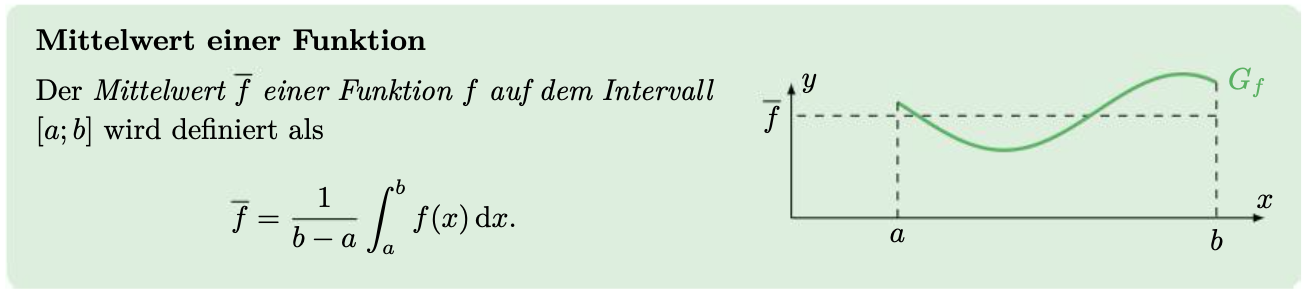
\includegraphics[width = \textwidth]{media/defMittelwert.png}
% \end{center}
% \end{definition}

% \begin{bsp}
%     {Mittelwert einer Funktion}{}
%     Der Mittelwert der Funktion $f(x)=x^2$ im Intervall $[0,1]$ ist:
%     $$ \bar{f} = \frac{1}{1-0}\int_0^1 x^2 \, dx = \frac{1}{3}$$
%     \begin{center}
%         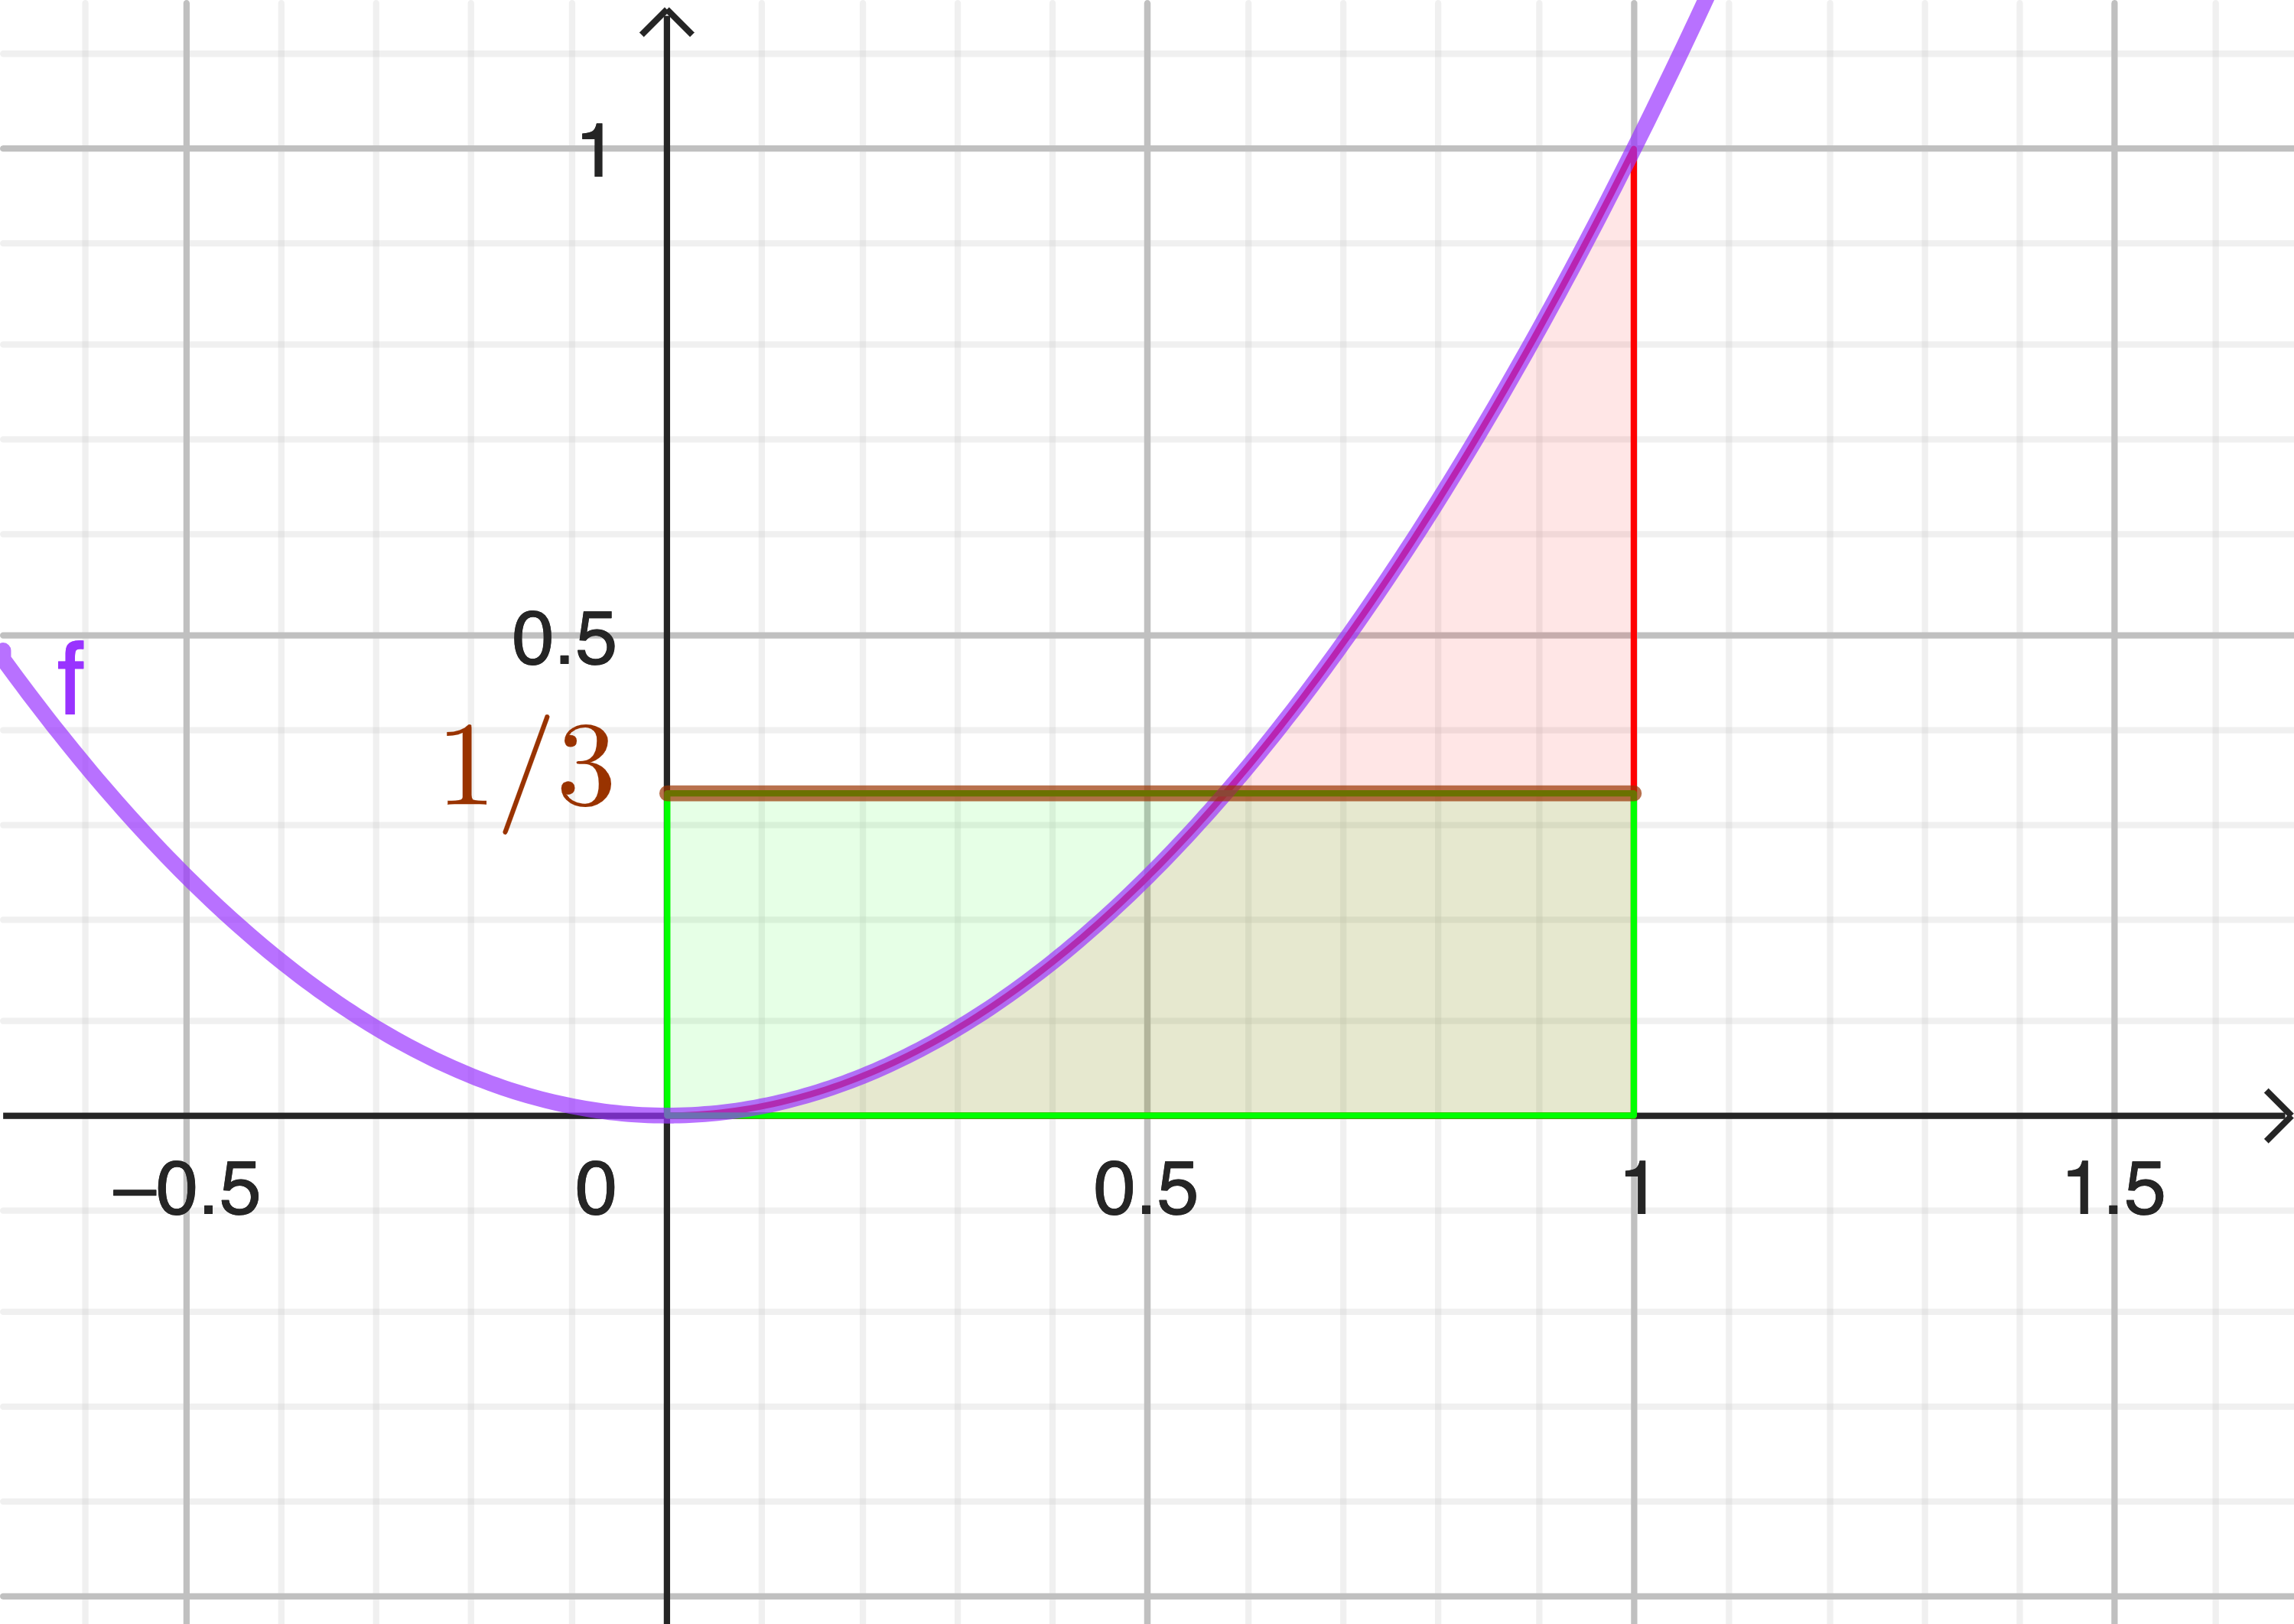
\includegraphics[width = 0.5 \textwidth]{media/bspMittelwert.png}
%     \end{center}
% \end{bsp}



